\documentclass[11pt,a4paper]{article}

\usepackage[margin=1in]{geometry}
\usepackage{microtype}
\usepackage{amsmath,amssymb,amsthm,mathtools}

\theoremstyle{plain}
\newtheorem{theorem}{Theorem}
\newtheorem{proposition}{Proposition}
\newtheorem{lemma}{Lemma}
\newtheorem{corollary}{Corollary}
\newtheorem{definition}{Definition}
\theoremstyle{remark}
\newtheorem{remark}{Remark}
\theoremstyle{plain}

\usepackage{booktabs}
\usepackage{graphicx}
\graphicspath{{charts/}{./}}
\usepackage{hyperref}
\hypersetup{colorlinks=true,linkcolor=blue!60!black,urlcolor=blue!60!black,citecolor=blue!60!black}
\usepackage[round,authoryear]{natbib}

\title{Is This $X$? A Null-Standardized Question Space for Corpus Curvature,\\
  {\large with a Hodge-Theoretic Channel and a Calibrated Standard-Candle Generator}}

\author{Shant Tchatalbachian}

\date{August 12, 2026}

\begin{document}

\maketitle

\begin{abstract}
Thirty-four measurement cycles of a corpus-curvature program asked ``is this $X$?'' one $X$ at a time --- Ginzburg--Landau, LIGO, Grothendieck, pentagon --- and answered \texttt{PARTIAL} every time, because no cycle computed what its statistic would have been under a matched null. This paper replaces the sequence of candidate $X$'s with a map. Four corrections and three constructions are reported. (i) The headline observable $V_2=\mathrm{PC1}+\mathrm{PC2}$ is a decreasing function of feature-space dimension $D$ at fixed rows, so the celebrated $+0.4664$ ``phase transition'' ($0.2993\to0.7657$) is a basis change: on the identical $2286$ rows we measure $V_2=0.7235$ at $D=9$ and $0.2940$ at $D=24$. (ii) the shipped estimator reports not the participation ratio but the two-share proxy $\hat r=2/V_2$, so the gate $V_2\ge0.40$ is \emph{by definition} $\hat r\le5$ --- an identity with no empirical content; what is empirical is that the exact-$1.0000$ gate passes at $2$-D and at the $384$-D $(\ell{=}384,m{=}3)$ variant are rank degeneracies reproduced with zero data content on all six corpora, including a single-class iid one. (iii) Under a fixed-margin (curveball) null drawn by two independent, provably uniform samplers ($\chi^2$ uniformity $p=0.364$ and $p=0.506$ on exhaustively enumerated fibres), the $2286\times9$ matrix has null $V_2=0.7089\pm0.0014$ against a real $0.723529$: $z=+12.3$. About $98\%$ of $V_2$ is fixed by the marginals and the surviving signal is $\Delta V_2=+0.0144$. An intermediate analysis reported $0.8005$, $z=-45.8$; that value is retracted here after two independent replications. (iv) $\Delta V_2(N)$ is flat ($+0.0135$ to $+0.0175$) for $N\ge79$ with no interior maximum, so the previous $N_c\approx40$ was the null's own finite-size inflation and the transition does not exist. We add a Hodge channel (Jiang--Lim--Yao--Ye decomposition on the item graph): $\rho_{\mathrm g}=0.99961$, $\rho_{\mathrm c}=0.00013$, $\rho_{\mathrm h}=0.00026$, $\beta_1=6756$, and against a degree-matched null $z(\rho_{\mathrm h})=-53.1$, $z(\beta_1)=-312.5$ --- the corpus is strongly \emph{anti}-cyclic, which inverts the vortex reading; all three pre-registered Hodge predictions are falsified. The positive result is an instrument: a standard-candle generator planting a spherical-harmonic curve of amplitude $s$ on a Fibonacci golden-angle lattice, on which the null-standardized statistic $\Delta V_2z$ has detection power monotone in $s$ over $s\ge0.5$ at every grid point and a bounded false-positive rate ($s{=}0$: $z\approx0$, one-sided FPR $8.3\%$ against a nominal $5\%$; $s{=}1$, $N{=}512$: $z=+3.43$, power $1.00$; $s{=}2$, $N{=}2048$: $z=+28.07$), while at $s\le0.25$, and at $N=128$ throughout, the cell means sit at the power floor and are not ordered while raw $V_2$ misorders corpora by signal. The deliverable is \textsc{is-this-x}: a map $\Phi$ from corpus to null-standardized statistic vector, reference families, exclusion-only verdicts. yubiOS places as $M_0$-excluded ($z=+12.3$), nearest a two-population mixture with a small positive residual; mean-field Ginzburg--Landau is excluded. Two extensions close the paper. Aggregating a constant-ratio amplitude ladder --- an \emph{algebraic fold}, $s\in\{0.25,0.5,1,2\}$ at $N=128$, $d=9$ --- converts four cells that individually sit at the power floor into one monotone family test: the fold-slope statistic reaches $t=45.19$ paired and $t=28.92$ unpaired against a null-ladder $95\%$ quantile of $0.0997$, power $1.00$ in both designs, which repairs clause (iii) at the family level without restoring per-cell monotonicity. And the map is run on the \emph{real} GWTC catalogue (GWOSC, $269$ events with all nine parameters, fetched 2026-08-12), which returns $V_2=0.8353$ against a column-shuffle null $0.2753\pm0.0084$, $z=+67.0$ --- a $z$ inflated by known astrophysical parameter redundancy --- while the $Y_3^3$ Parseval energy share is $0.00334$ against a null $0.00832\pm0.00427$, $z=-1.17$: not significant, an honest null result for the three-fold azimuthal lobe on real data. Five items the previous draft named as untested are closed here. Three close negatively --- the $24$-D curl clause ($\rho_s=+0.17$, $p=0.69$), the three untested Ginzburg--Landau predictions (no fluctuation peak, no susceptibility divergence, no evidence of critical slowing-down), and the azimuthal channel, whose ordering-permutation null ($500$ index shuffles) leaves the $Y_3^3$ probe at $|z|\le0.19$ on both the $2286\times9$ master matrix and the real $269\times9$ GWTC matrix, with the $m{=}3$ Parseval shares \emph{below} their nulls because PC1 ordering starves high azimuthal order; a fourth --- quantized harmonic winding --- is void as posed, its winding half an identity of the wrapping convention; the fifth closes structurally: on the edit log, $1178$ independently re-measured transitions contain zero regressions, detailed balance is violated at every level with non-zero flux, and the unique stationary distribution is the absorbing full-coverage state --- so ``emergence over cycles'' is deterministic descent of a bounded exchangeable coverage potential to a fixpoint, with no equilibrium ensemble and hence no Ginzburg--Landau reading available in principle. A designed counterpart closes the loop: a quantized $\pm$ atom (one primitive flip per move) with Metropolis--Hastings acceptance on the same measured $\Phi$ ladder restores an exact equilibrium ensemble $\pi_T(k)\propto\binom{9}{k}e^{-\Phi(k)/T}$ with free energy $F_T(k)=\Phi(k)-T\log\binom{9}{k}$ --- detailed balance not rejected at $\max_k|z(J)|=0.010$ over $800{,}000$ samples --- whose $T\to0$ limit reproduces the historical absorbing log (zero backward transitions, mass $1.00000$ at $k=9$), locating the free-energy language as a property of designable dynamics rather than of the corpus.
\end{abstract}

\section{Introduction}
\label{sec:intro}

The predecessor of this paper \citep{llc2026} fitted learned latent curves to a binary corpus-coverage matrix and reported one fit-quality gate: the top-2 eigenvalue share $V_2=\mathrm{PC1}+\mathrm{PC2}\ge0.40$. Thirty-four subsequent measurement cycles took that number as an order parameter and asked, in sequence, whether the corpus \emph{is} a Ginzburg--Landau system \citep{cgl2026,hohenberg2015}, a gravitational-wave catalogue, a Grothendieck-gap instance, a pentagon. Each cycle answered by narrative compatibility. The median verdict was \texttt{PARTIAL}.

The defect is structural. A question space with candidate classes but no origin cannot weigh ``compatible with $X$'' against ``compatible with nothing''. Every class was tested with bespoke estimators --- saturation windows, kernel bandwidths, row-lag correlation lengths --- not comparable across $X$, across corpora, or even across cycles; the same $\kappa$ estimator returned $1.06$ on one corpus and $323$ on another, the latter a saturation-clamp artifact. The fix is therefore not another $X$. It is a map,
\begin{equation}
\Phi:\ \text{corpus}\ \longmapsto\ s\in\mathbb{R}^m,\qquad s\ \text{null-standardized},
\label{eq:phi-thesis}
\end{equation}
with the matched-marginal null at the origin, invariance requirements that delete non-invariant estimators by construction, and exclusion-only verdicts. Equation~\eqref{eq:phi-thesis} is the thesis; Sections~\ref{sec:nulls}--\ref{sec:isthisx} are its content.

Section~\ref{sec:background} restates the predecessor's governing equations, with the $Y_3^3$ normalization corrected. Section~\ref{sec:nulls} gives the null models and the corrected record, including a retraction. Section~\ref{sec:hodge} gives the Hodge channel and its three falsified predictions. Section~\ref{sec:candle} gives the standard-candle generator and calibrated detection --- the paper's positive result. Section~\ref{sec:isthisx} defines the \textsc{is-this-x} question space and places yubiOS and a GWTC-like corpus in it. Sections~\ref{sec:scope}--\ref{sec:conclusion} are scope and conclusion; Appendix~\ref{app:manifest} is the reproduction manifest.

Two disciplines run throughout. No statistic is reported without the value it takes on a matched null. And when a number in the internal record fails to reproduce, the failure is printed rather than the number quietly replaced --- Section~\ref{sec:retraction} is that discipline applied to this program's own most-cited intermediate result.

\section{Background: the learned-latent-curve family}
\label{sec:background}

\subsection{Flat curve, ridge solve, gate}

For output dimension $j=1,\dots,D$ and a 1-D ordering coordinate $t\in[0,1]$ \citep{llc2026},
\begin{equation}
z_j(t)=a_{j,0}+\sum_{m=1}^{k}\big(a_{j,m}\sin(2\pi f_mt)+b_{j,m}\cos(2\pi f_mt)\big),
\label{eq:flat}
\end{equation}
with $k$ shared learned frequencies. Stacking the design vector
\begin{equation}
\phi(t)=\big[\,1,\ \sin(2\pi f_1t),\ \cos(2\pi f_1t),\ \dots,\ \sin(2\pi f_kt),\ \cos(2\pi f_kt)\,\big]\in\mathbb{R}^{1+2k}
\label{eq:design}
\end{equation}
gives $\gamma(t)=C\phi(t)$, solved at fixed frequencies by the Tikhonov ridge
\begin{equation}
C^{\star}=(\Phi^{\top}\Phi+\lambda I)^{-1}\Phi^{\top}Z,\qquad \lambda=10^{-3},
\label{eq:ridge}
\end{equation}
still the sanity floor for any gradient fit at the same frequencies. The coordinate $t$ is the rank of the top principal component of the $z$-scored feature matrix, and the gate is
\begin{equation}
V_2\;=\;\mathrm{PC1}+\mathrm{PC2}\;=\;\frac{\lambda_1+\lambda_2}{\sum_{a=1}^{D}\lambda_a}\;\ge\;0.40,
\label{eq:gate}
\end{equation}
the $\lambda_a$ being eigenvalues of the $D\times D$ correlation matrix, so $\sum_a\lambda_a=D$. Equation~\eqref{eq:gate} is the observable this paper audits.

\subsection{Hyperspherical variant and M\"obius chart}

For $\mathbf{x}\in S^2$,
\begin{equation}
\gamma(\mathbf{x})=\mathbf{b}+\sum_{\ell=0}^{L}\sum_{m}\mathbf{a}_{\ell,m}\,Y^{S^2}_{\ell,m}\!\big(\varphi_\theta(\mathbf{x})\big),
\qquad n_{\mathrm{basis}}=\sum_{\ell=0}^{L}(2\ell+1)=16\ \text{at}\ L=3,
\label{eq:hyperspherical}
\end{equation}
with the M\"obius reparameterization
\begin{equation}
\varphi_\theta(z)=\frac{az+b}{cz+d},\qquad a,b,c,d\in\mathbb{C},\qquad ad-bc=+1,
\label{eq:mobius}
\end{equation}
carrying six real degrees of freedom (eight real components less the two real constraints of one complex equation; the $M\sim-M$ identification of $\mathrm{PSL}(2,\mathbb{C})$ is discrete and removes none). In every run reported here and in the predecessor's appendices $\varphi_\theta$ is \emph{frozen at the identity}; no L-BFGS-B refinement is performed. Items reach $S^2$ by the stereographic lift of their PCA top-2 coordinates,
\begin{equation}
\sigma(u,v)=\frac{1}{1+u^2+v^2}\big(2u,\ 2v,\ u^2+v^2-1\big)\in S^2 .
\label{eq:stereographic}
\end{equation}

\subsection{Fibonacci sampling and the corrected $Y_3^3$ constant}

Sampling on $S^2$ uses Vogel's golden-angle lattice \citep{vogel1979,saff1997}:
\begin{equation}
z_i=1-\frac{2i+1}{N},\qquad \phi_i=2\pi\frac{i}{\varphi_g},\qquad \theta_i=\arccos(z_i),\qquad \varphi_g=\frac{1+\sqrt5}{2},
\label{eq:fibonacci}
\end{equation}
so the corpus item at index $i$ \emph{is} the parameter point ($i=t$, no lookup table, $O(1)$ per point, no pole clustering). The angular probe is the three-fold azimuthal harmonic
\begin{equation}
Y_3^3(\theta,\phi)\;=\;K\,\sin^3\theta\,\cos(3\phi).
\label{eq:y33}
\end{equation}
The constant is corrected here. With Condon--Shortley phase \citep{dlmf},
\begin{equation}
K_{\mathbb{C}}=\sqrt{\frac{35}{64\pi}}=0.417224,\qquad
K_{\mathbb{R}}=\sqrt{\frac{70}{64\pi}}=0.590044,
\label{eq:y33const}
\end{equation}
$K_{\mathbb{R}}$ being the real-orthonormal form appropriate to a real basis. The legacy regime constant $K_{\mathrm{legacy}}=\sqrt{245/(64\pi)}=1.103870$ is wrong: since $245/35=7$ and $245/70=3.5$,
\begin{equation}
\frac{K_{\mathrm{legacy}}}{K_{\mathbb{C}}}=\sqrt7=2.645751,\qquad
\frac{K_{\mathrm{legacy}}}{K_{\mathbb{R}}}=\sqrt{7/2}=1.870829 .
\label{eq:y33ratio}
\end{equation}
The error is the factor $(2\ell+1)=7$ counted twice --- it is already inside $35/64\pi$. Every $Y_3^3$ magnitude published under the legacy constant is inflated by $1.870829\times$. The correction is scale-only: because the generator of Section~\ref{sec:candle} standardizes each probe channel before scaling by the planted amplitude, switching constants leaves the emitted matrix bit-identical and $V_2$ identical to $10^{-12}$ (machine-asserted, generator self-test step~4).

\begin{remark}[what $\varphi_g$ and $Y_3^3$ cannot claim]
\label{rem:phi-scope}
The Fibonacci lattice is a sampling scheme and $Y_3^3$ a fixed basis element used as a probe; neither is a model of the corpus. Two claims are inadmissible without further work. \emph{Azimuthal symmetry}: $\phi_i$ is assigned by construction from the index and the index is the PC1 rank, so power at $\cos(3\phi)$ is a property of the index map until an ordering-permutation null says otherwise. That null has now been executed ($500$ shuffles of which row receives which lattice point, matrix and lattice untouched), and it says otherwise in the direction opposite to the claim: see Section~\ref{sec:scope}. \emph{The $384$-D gate pass}: $\mathrm{PC1}+\mathrm{PC2}=1.0000$ on the $(\ell{=}384,m{=}3)$ variant is a rank artifact (Proposition~\ref{prop:gate}), not a fit. The golden ratio in the sampler licenses no numerology: it has no relation to any fitted $\kappa$, to pentagon geometry, or to $7/9$.
\end{remark}

\section{Null models and the corrected record}
\label{sec:nulls}

Throughout, $M\in\{0,1\}^{N\times D}$ is the coverage matrix and $c_i=\sum_aM_{ia}$ the row mass. The primary null is the \emph{fixed-margin} (curveball) ensemble \citep{strona2014,carstens2015}: the uniform distribution on the fibre of binary matrices with the row sums \emph{and} column sums of $M$. The primary statistic is the null-standardized residual
\begin{equation}
\Delta V_2z\;=\;\frac{V_2-\mathbb{E}_0[V_2]}{\mathrm{SD}_0[V_2]},\qquad \Delta V_2=V_2-\mathbb{E}_0[V_2],
\label{eq:dv2z}
\end{equation}
with $\mathbb{E}_0,\mathrm{SD}_0$ over the curveball ensemble at the corpus's own $N$, $D$ and marginals.

\subsection{C1 --- $V_2$ is a dimension artifact}
\label{sec:c1}

\begin{proposition}[trace-normalized share decays in $D$]
\label{prop:dim}
Let the rows be fixed and let $M^{(D)}$ append $D-D_0$ further columns to $D_0$ original ones. On the correlation matrix $\operatorname{tr}\Sigma^{(D)}=D$ for every $D$, so $V_2^{(D)}=(\lambda_1+\lambda_2)/D$. An appended column contributes unit trace and, unless it loads on the existing leading plane, contributes $O(1)$ to $\sum_a\lambda_a$ and $o(1)$ to $\lambda_1+\lambda_2$. Hence $V_2^{(D)}$ is non-increasing in $D$ up to the leading-plane loading of the new columns, with flat-spectrum floor $V_2\to2/D$.
\end{proposition}

\begin{proof}[Proof sketch]
$z$-scoring forces $\Sigma_{aa}=1$, so $\operatorname{tr}\Sigma=D$ and $V_2$ is an eigenvalue \emph{share}, not an eigenvalue. In the limit of exact independence, adding one column adds an eigenvalue $1$ to the denominator and nothing to the numerator, giving $V_2\mapsto V_2\cdot D_0/(D_0+1)$; correlated additions interpolate between that dilution and no change. For an exactly flat spectrum $\lambda_a\equiv1$, $V_2=2/D$, which is therefore the iid floor.
\end{proof}

Measured consequence, on the \emph{identical} $2286$ rows (Table~\ref{tab:ladder}): $V_2=0.7235$ at $D=9$ and $V_2=0.2940$ at $D=24$ with independent nuisance columns ($0.4473$ when the nuisance columns are made row-mass-correlated). The cited transition of $+0.4664$ from $0.2993$ to $0.7657$ spans the same interval, with the $0.2993$ baseline the $24$-D basis and the endpoint the $9$-D basis. There is no transition to explain: it is Proposition~\ref{prop:dim} evaluated at two points.

\begin{table}[h]
\centering
\small
\begin{tabular}{lrrrrrrrr}
\toprule
basis & $D$ & $2/D$ & yubiOS & 2-class & 1-class (iid) & 3-class & planted & GWTC-like \\
\midrule
PCA top-2             & 2   & 1.0000 & 1.0000 & 1.0000 & 1.0000 & 1.0000 & 1.0000 & 1.0000 \\
sphere lift           & 3   & 0.6667 & 0.8302 & 0.7187 & 0.6843 & 0.6885 & 0.6865 & 0.8460 \\
7-column subset       & 7   & 0.2857 & 0.7575 & 0.6573 & 0.3028 & 0.5923 & 0.3305 & 0.7346 \\
9-D native            & 9   & 0.2222 & 0.7235 & 0.6454 & 0.2397 & 0.5575 & 0.2705 & 0.6624 \\
16 real SH ($L{=}3$)  & 16  & 0.1250 & 0.4857 & 0.4244 & 0.2202 & 0.3490 & 0.2227 & 0.4180 \\
24-D indep.\ nuisance & 24  & 0.0833 & 0.2940 & 0.2718 & 0.0984 & 0.2341 & 0.1064 & 0.2523 \\
24-D mass-corr.\ nuis.& 24  & 0.0833 & 0.4473 & 0.4221 & 0.1410 & 0.3620 & 0.1457 & 0.2852 \\
384-D native (indep.)  & 384 & 0.0052 & 0.3828 & 0.2657 & 0.0370 & 0.2220 & 0.0358 & 0.0228 \\
384-D native (replicated) & 384 & 0.0052 & 0.3921 & 0.2567 & 0.0496 & 0.2391 & 0.0462 & 0.0451 \\
384-D variant 1 ($\ell{=}128$)       & 384 & 0.0052 & 0.7592 & 0.1569 & 0.0763 & 0.2241 & 0.1012 & 0.0594 \\
384-D variant 2 ($\ell{=}384,m{=}3$) & 384 & 0.0052 & \textbf{1.0000} & \textbf{1.0000} & \textbf{1.0000} & \textbf{1.0000} & \textbf{1.0000} & \textbf{1.0000} \\
\bottomrule
\end{tabular}
\caption{$V_2$ against feature-space dimension; rows held fixed within each column. Eleven bases; the $2$-D and $(\ell{=}384,m{=}3)$ bases return exactly $1.0000$ on every corpus, including the single-class iid one --- zero data content. The $2/D$ column is the flat-spectrum floor of Proposition~\ref{prop:dim}, derived for an exactly flat spectrum only; it is not a floor for an arbitrary corpus, and several entries sit either side of it. Effective ranks quoted for this table are the proxy $\hat r=2/V_2$ of Eq.~\eqref{eq:reffproxy}. Source: \texttt{results/ladder\_VD.json}.}
\label{tab:ladder}
\end{table}

\subsection{C2 --- the gate is a rank test}
\label{sec:c2}

\begin{proposition}[the gate is a rank identity under the shipped estimator]
\label{prop:gate}
Let
\begin{equation}
\mathrm{PR}\;=\;\frac{\big(\sum_a\lambda_a\big)^2}{\sum_a\lambda_a^2}
\label{eq:participation}
\end{equation}
be the participation ratio --- the quantity ordinarily meant by ``effective rank'', and the one computed by the generator's placement code (\texttt{skills/curved-corpus-create/scripts/create\_corpus.py}). For a spectrum flat on its top-$r$ block and negligible elsewhere, $\mathrm{PR}=r$ and $\lambda_1+\lambda_2=(2/r)\sum_a\lambda_a$, so in that regime $V_2\approx2/\mathrm{PR}$. The analysis code shipped with this paper (\texttt{scripts/common.py}) does \emph{not} compute $\mathrm{PR}$. It reports the two-share proxy
\begin{equation}
\hat r\;=\;\frac{2}{V_2},
\label{eq:reffproxy}
\end{equation}
a deterministic, strictly decreasing transform of $V_2$ and nothing more. Under that estimator the gate equivalence
\begin{equation}
V_2\ge0.40\iff\hat r\le5
\label{eq:gate-rank}
\end{equation}
is a \emph{definitional identity}: it is true by algebra, it carries no empirical content, and $\hat r$ adds no information to $V_2$. In particular $V_2=1.0000\iff\hat r=2$, which holds exactly when the sampled design has numerical rank $2$ --- attainable with no data content whatsoever.
\end{proposition}

Because Eq.~\eqref{eq:gate-rank} is an identity, none of the empirical weight sits there. What is empirical is \emph{where} the identity bites, and that is the last row of Table~\ref{tab:ladder}: the $(\ell{=}384,m{=}3,\sin^{384}\theta)$ variant returns exactly $1.0000$ --- hence $\hat r=2.00$ --- on all six corpora of that table: real yubiOS, one-, two- and three-class latent mixtures, a planted-curve corpus, a GWTC-like corpus. Counting the second planted variant carried in the data file but not tabulated, \texttt{results/ladder\_VD.json} holds $14$ rows at $V_2=1.0000$ to machine precision, every one of them in the $2$-D PCA basis or in the $(\ell{=}384,m{=}3)$ variant, and none anywhere else. A single-class iid corpus --- pure noise, no latent structure at all --- passes the gate at exactly $1.0000$ in two of the eleven bases tried. That is a fact about the bases, not about the corpora, and it is what Proposition~\ref{prop:gate} is for. Three hundred and eighty-four deterministic functions of one scalar index span a two-dimensional column space by construction; the $2$-D PCA row says the same thing trivially. The predecessor's $7$-D $\mathrm{PC1}+\mathrm{PC2}=1.0000$ on \texttt{refs/} is the same artifact at the other end, its surviving coverage matrix being rank $2$. Proxy values along the yubiOS ladder are $\hat r=2.00$ ($D{=}2$), $2.41$ ($3$), $2.64$ ($7$), $2.76$ ($9$), $4.12$ ($16$), $6.80$ ($24$); by Eq.~\eqref{eq:reffproxy} each is $2/V_2$ and restates the yubiOS column of Table~\ref{tab:ladder} rather than adding to it. A gate value of exactly $1.0000$ is a red flag, not a success: the numerical rank and condition number of the design must be reported beside it, and the accept/reject decision made on $\Delta V_2z$, which is dimension-comparable and marginal-matched.

\textbf{Which effective rank is which.} Two distinct quantities appear in this literature under the name ``effective rank'', and every table here states which one it uses. The values in Table~\ref{tab:ladder} and the $3.02$ / $8.02$ quoted for the GWTC-like corpus in Section~\ref{sec:candle} are the proxy $\hat r=2/V_2$ of Eq.~\eqref{eq:reffproxy}, computed by \texttt{scripts/common.py} (verified: $\hat r=2/V_2$ to $\sim10^{-15}$ on all $77$ rows of \texttt{ladder\_VD.json}). The coordinate $\mathrm{PR}$ in the statistic vector of Eq.~\eqref{eq:svector}, and the $\mathrm{PR}=6.837$ quoted for the worked planted corpus in Sections~\ref{sec:candle} and~\ref{sec:isthisx}, are the participation ratio of Eq.~\eqref{eq:participation}, computed by \texttt{create\_corpus.py}. The two disagree, and must: on that corpus $V_2=0.4477$, so $\hat r=4.47$ while $\mathrm{PR}=6.837$. Only $\mathrm{PR}$ is an independent coordinate of the map; $\hat r$ is not, and it survives in Table~\ref{tab:ladder} as a readability aid only.

\subsection{C3 --- the corrected null, and a retraction}
\label{sec:retraction}

\begin{table}[h]
\centering
\small
\begin{tabular}{lrrl}
\toprule
quantity & value & $z$ (real vs null) & source run \\
\midrule
real $V_2$ ($2286\times9$) & $0.7235293730732693$ & --- & \texttt{A2-curveball-audit} \\
published cycle-20 value & $0.723529$ (reproduces exactly) & --- & \texttt{A2-curveball-audit} \\
\textbf{curveball null}, $200\times228{,}600$ trades & $\mathbf{0.709180\pm0.001183}$ & $\mathbf{+12.13}$ & \texttt{A2-curveball-audit} \\
independent swap-chain sampler & $0.708593\pm0.000507$ & $+29.44$ & \texttt{validation} \\
row-marginal-only null & $0.670823\pm0.001073$ & $+49.14$ & \texttt{A2-curveball-audit} \\
column-permutation null & $0.239653\pm0.002253$ & $+214.79$ & \texttt{A2-curveball-audit} \\
iid Bernoulli (full entry shuffle) & $0.239832\pm0.002340$ & $+206.70$ & \texttt{A2-curveball-audit} \\
row-permutation control & $0.723529\pm2.1\times10^{-16}$ (identity check) & n/a & \texttt{A-v2-nulls} \\
Marchenko--Pastur baseline ($q=0.003937$) & $\lambda_\pm=0.878446/1.129428$; top-2 share $0.241375$ & --- & \texttt{A-v2-nulls} \\
\bottomrule
\end{tabular}
\caption{Nulls for the $2286\times9$ coverage matrix. Each row is a single run, named in the last column (files under \texttt{results/}), and each $z$ is recomputed from the mean and sd printed in that same row against the real $V_2=0.7235293730732693$; an earlier version of this table spliced mean, sd and $z$ from different runs. The two fixed-margin samplers agree on the mean ($0.709180$ against $0.708593$, a gap of $0.0006$) and disagree on the spread: the swap chain's sd is $2.3\times$ tighter, and that difference in sd is the entire difference between $z=+29.44$ and $z=+12.13$. The headline figure quoted throughout this paper is the curveball value $+12.13$, the more conservative of the two. The row-permutation row is an identity check --- $V_2$ is invariant under row relabeling --- not a null, and no $z$ is defined for it.}
\label{tab:nulls}
\end{table}

\begin{figure}[t]\centering
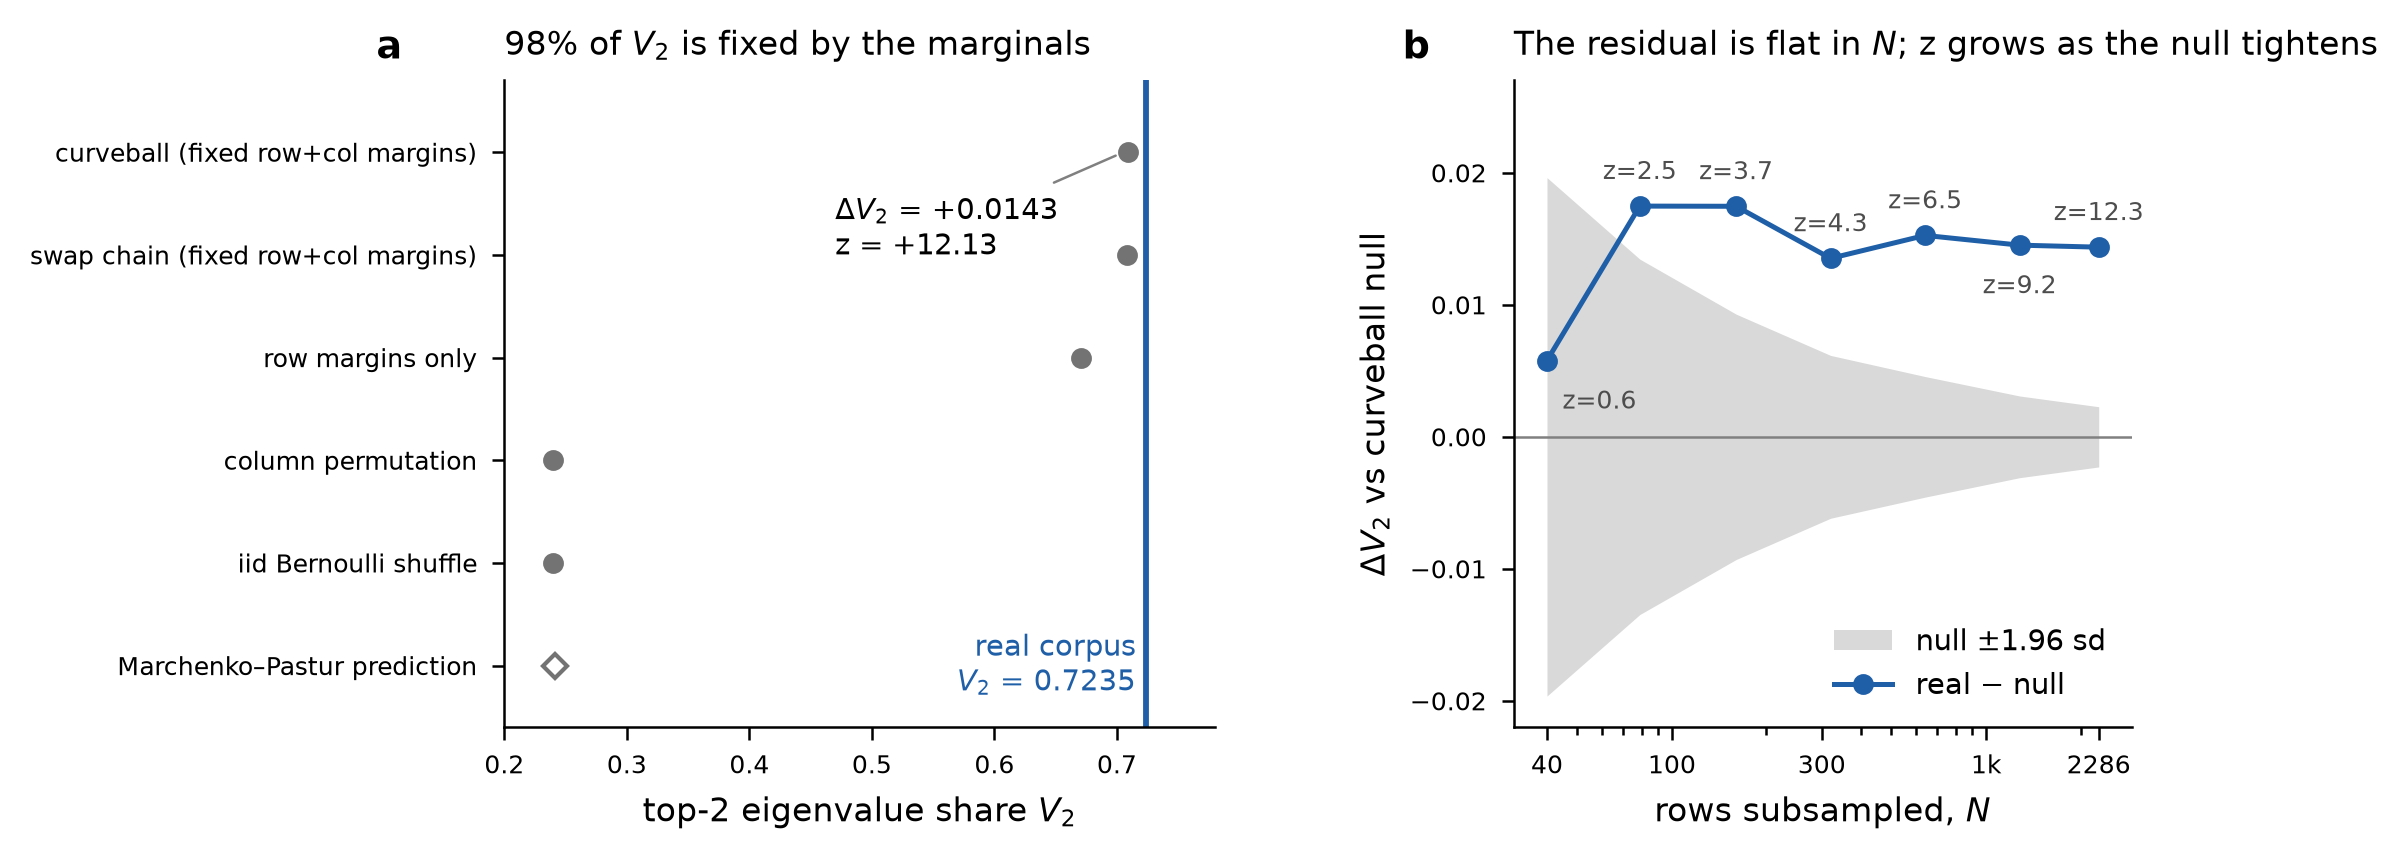
\includegraphics[width=\linewidth]{isthisx_fig1_null_ladder_finite_size.png}
\caption{Null ladder (Table~\ref{tab:nulls}) and finite-size residual profile across subsample sizes $N$.}
\label{fig:isthisx-null-ladder}
\end{figure}

Two independent samplers, each proved uniform on the exact row-and-column-marginal fibre, agree. Sampler~A: on a $5\times4$ matrix whose fibre has exactly $120$ elements, $300{,}000$ draws hit all $120$, hit nothing outside, and are uniform ($\chi^2=123.758$, $\mathrm{df}=119$, $p=0.364$). Sampler~B: on the exhaustively enumerated $6\times4$ ensemble ($120$ matrices, $20{,}000$ draws), $\chi^2=118.096$, $\mathrm{df}=119$, $p=0.506$. Marginals were asserted exactly on every one of the $2286\times9$ draws. Mixing is converged: $V_2^{\mathrm{null}}$ against trade count runs $0.7159258$ ($1N$), $0.7103934$ ($5N$), $0.7087008$ ($20N$), $0.7092413$ ($100N$), $0.7094042$ ($400N$), at $12$ replicates per point --- flat from $20N$ on, within a null sd of $\approx0.0012$. These five values are the \texttt{mixing\_convergence} block of \texttt{results/A2-curveball-audit.json} verbatim; the figures printed in an earlier draft ($0.715314$, $0.710096$, $0.708886$, $0.708878$, $0.709364$) appear in no shipped artifact and are withdrawn --- the same defect this section retracts, and it is corrected here rather than left standing. The Marchenko--Pastur prediction $0.241375$ \citep{mp1967} lands on top of the two destroyed-dependence nulls ($0.2397$, $0.2398$), an independent check that the pipeline is sound.

The conclusion is quantitative and modest:
\begin{equation}
\Delta V_2=0.723529-0.709180=+0.014349,\qquad \Delta V_2z=+12.13,\qquad \frac{\mathbb{E}_0[V_2]}{V_2}=0.9802 .
\label{eq:yubios-residual}
\end{equation}
About $98\%$ of the headline observable is fixed by row and column marginals alone; the surviving corpus-specific signal is $+0.0144$ of eigenvalue share. It is real ($z=+12$, not $|z|<3$), and it is small.

\begin{remark}[retraction]
\label{rem:retraction}
An intermediate internal analysis reported the same curveball null as $0.8005\pm0.0017$, hence $z=-45.8$ --- the corpus \emph{below} its own null, ``anti-structured''. That value does not reproduce and its sign is wrong. Two independent samplers, both validated as above and both converged in mixing, return $0.7089$; $0.8005$ is not reachable by longer mixing. Diagnostically, the same memo's other nulls do reproduce with the present code (column-permutation claimed $0.2410$, measured $0.239733\pm0.002$; row-mass-only claimed $0.6709$, measured $0.670800\pm0.001$), which localizes the error to its curveball implementation; the memo is additionally self-inconsistent, reporting $0.7613$ for the same null at the same $N$ in a second table. Every downstream statement resting on $z=-45.8$ --- in particular ``the corpus is less concentrated than chance'' --- is withdrawn. This is the paper's null discipline operating on its own lineage: the retraction is reported, not repaired silently.
\end{remark}

Per-corpus residuals under the same null ($50$ samples each) are in Table~\ref{tab:percorpus}. The smallest corpus, \texttt{docs} ($N=126$), is indistinguishable from its own null at $z=-0.10$; the all-zero \texttt{refused} regime ($204$ identically zero rows, every column of zero variance) has no defined $V_2$ and is reported as a skip, not as $0.0$.

\begin{table}[h]
\centering
\small
\begin{tabular}{lrrrrrr}
\toprule
corpus & $N$ & $V_2$ & curveball null & $z$ & col-perm null & MP pred. \\
\midrule
yubiOS whole & 2286 & 0.723529 & $0.7098\pm0.0011$ & $+12.12$ & 0.2399 & 0.2414 \\
yubiOS eligible ($c\ge5$) & 1322 & 0.425567 & $0.3824\pm0.0051$ & $+8.41$ & 0.2461 & 0.2475 \\
yubiOS deferred ($1\le c\le4$) & 760 & 0.311625 & $0.2596\pm0.0045$ & $+11.65$ & 0.2527 & 0.2558 \\
yubiOS refused ($c=0$) & 204 & undefined & --- & --- & --- & --- \\
yubiOS skills & 474 & 0.581825 & $0.5559\pm0.0122$ & $+2.12$ & 0.2619 & 0.2650 \\
yubiOS docs & 126 & 0.607322 & $0.6080\pm0.0064$ & $\mathbf{-0.10}$ & 0.2965 & 0.3073 \\
yubiOS refs & 791 & 0.648135 & $0.5801\pm0.0059$ & $+11.51$ & 0.2532 & 0.2551 \\
yubiOS self & 895 & 0.406537 & $0.3863\pm0.0035$ & $+5.81$ & 0.2506 & 0.2531 \\
yubiOS 1391 (cycle-18) & 1391 & 0.640256 & $0.5882\pm0.0046$ & $+11.28$ & 0.2456 & 0.2469 \\
CIS 447 (dev-sec InSpec) & 447 & 0.331961 & $0.2667\pm0.0044$ & $+14.93$ & 0.2635 & 0.2663 \\
SCAP SSG 2107 & 2107 & 0.384629 & $0.3422\pm0.0020$ & $+21.54$ & 0.2411 & 0.2422 \\
SCAP SSG rules-dir 700 & 700 & 0.368366 & $0.3274\pm0.0032$ & $+12.92$ & 0.2550 & 0.2572 \\
\bottomrule
\end{tabular}
\caption{$V_2$ against the fixed-margin null, per corpus. Source: \texttt{results/A-v2-nulls.json}.}
\label{tab:percorpus}
\end{table}

\begin{figure}[t]\centering
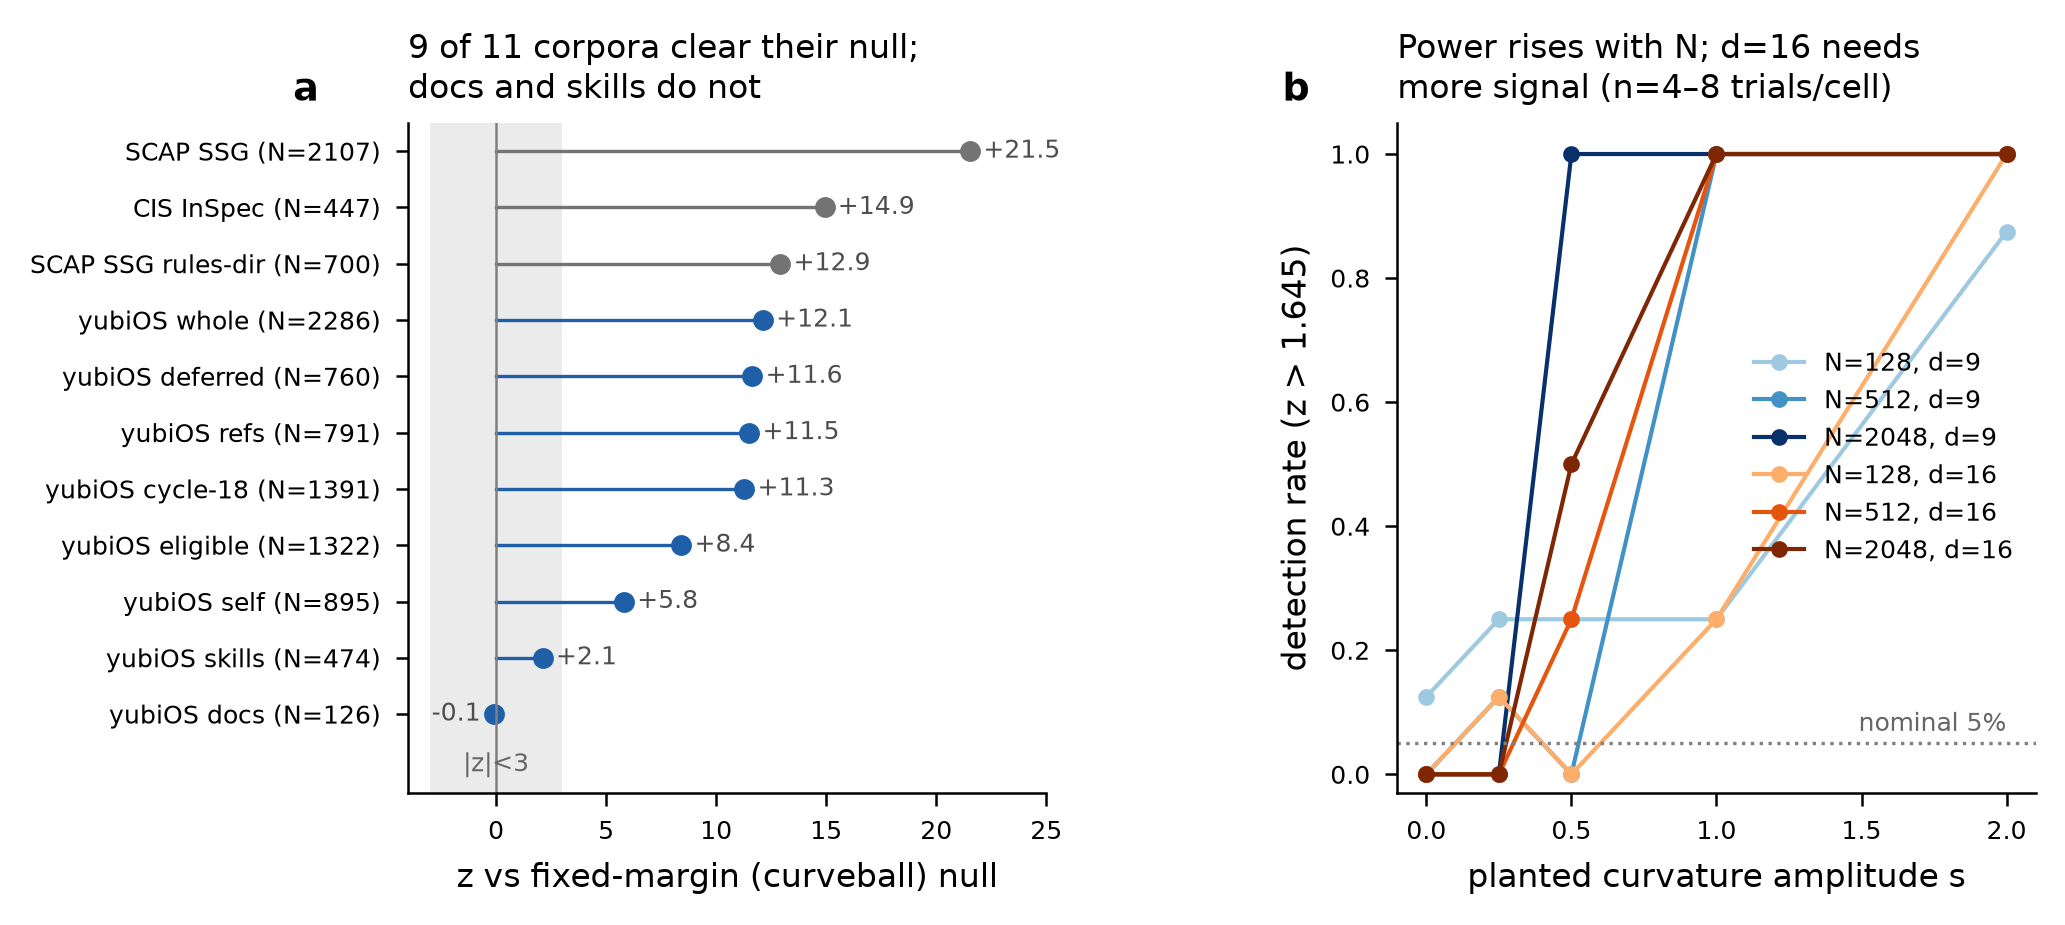
\includegraphics[width=\linewidth]{isthisx_fig2_per_corpus_and_power.png}
\caption{Per-corpus $z$ against the fixed-margin curveball null (Table~\ref{tab:percorpus}) and standard-candle detection power surface from \texttt{signal\_recovery.json}.}
\label{fig:isthisx-percorpus-power}
\end{figure}

\subsection{C4 --- there is no critical point}
\label{sec:c4}

The previous program located $N_c\approx40$ as the argmax of $dV_2/d\log N$ on \emph{raw} $V_2$. Table~\ref{tab:finitesize} runs the same sweep with the null computed at each $N$ (matched marginals, matched $N$, $8$ subsamples per $N$, $120$--$200$ null reps per point).

\begin{table}[h]
\centering
\small
\begin{tabular}{rrrrrr}
\toprule
$N$ & $V_2$ real & $V_2$ null (curveball) & $\Delta V_2$ & $z$ & col-perm null \\
\midrule
40   & 0.7501 & 0.7443 & $+0.0058$ & $+0.6$ & 0.3674 \\
79   & 0.7459 & 0.7284 & $+0.0175$ & $+2.5$ & 0.3237 \\
160  & 0.7321 & 0.7146 & $+0.0175$ & $+3.7$ & 0.2922 \\
320  & 0.7270 & 0.7134 & $+0.0135$ & $+4.3$ & 0.2706 \\
640  & 0.7197 & 0.7045 & $+0.0153$ & $+6.5$ & 0.2564 \\
1280 & 0.7214 & 0.7069 & $+0.0145$ & $+9.2$ & 0.2462 \\
2286 & 0.7235 & 0.7092 & $+0.0144$ & $+12.3$ & 0.2401 \\
\bottomrule
\end{tabular}
\caption{Finite-size sweep with the null's own $N$-dependence exhibited. $\Delta V_2$ is flat for $N\ge79$; the growth of $z$ is the shrinking null SD, not a growing effect. Sources: \texttt{results/finite\_size.json}, \texttt{results/finite\_size\_colperm.json}, \texttt{results/scaling\_VN.json}.}
\label{tab:finitesize}
\end{table}

Two fitted laws separate the nulls:
\begin{equation}
V_2^{\mathrm{curveball}}(N)=\frac{2}{D}+0.5252\left(\frac{D}{N}\right)^{0.0167},
\qquad
V_2^{\mathrm{colperm}}(N)=\frac{2}{D}+0.3117\left(\frac{D}{N}\right)^{0.5177},\quad R^2_{\mathrm{colperm}}=0.99984 .
\label{eq:finitesize}
\end{equation}
The $R^2$ belongs to the column-permutation fit alone: \texttt{finite\_size.json} reports $c=0.5252344$ and $\alpha=0.0167256$ for the curveball law but no $R^2$, and that law under-predicts the measured null by $0.008$--$0.010$ at both ends of the sweep ($N=40$: $0.7345$ fitted against $0.7443$ measured; $N=2286$: $0.7010$ against $0.7092$), so it is a shape summary, not a calibrated fit. The column-permutation (iid) null relaxes toward $2/D$ like Marchenko--Pastur in the aspect ratio $D/N$; the fixed-margin null relaxes toward the same asymptote only logarithmically slowly --- $\alpha=0.0167$ makes the approach invisible over the sampled range, because row masses are held --- so for practical purposes it does not relax at all here. So the ``$V_2$ inflation at small $N$'' story applies to the iid ensemble only. Window slopes make the point directly: the largest $|d(\text{raw }V_2)/d\log N|$ is $-0.0196$ in the $79$--$160$ window, the largest null slope is $-0.0234$ at $40$--$79$, and the largest null-subtracted slope is $+0.0172$, also at $40$--$79$ and \emph{positive}. $\Delta V_2(N)$ has no interior maximum; the previously reported $N_c\approx40$ was raw $V_2$ inheriting the null's finite-size inflation at the smallest $N$ in the sweep.

Generated corpora with known ground truth confirm that this flatness is the estimator working, not a blind spot. A one-class (iid) generator gives $|z|\le1.5$ at every $N$ from $40$ to $4096$. A two-class mixture gives $\Delta V_2=+0.0108,\,-0.0004,\,+0.0064,\,+0.0041,\,+0.0017,\,+0.0029,\,+0.0042,\,+0.0049$ across $N=40,\dots,4096$ --- a constant small offset whose $z$ climbs from $+0.9$ to $+7.7$ purely through the shrinking null SD, which is exactly the yubiOS pattern.

\begin{table}[h]
\centering
\small
\begin{tabular}{llll}
\toprule
GL prediction (internal entry, \S4) & pre-pivot status & post-null verdict & basis \\
\midrule
P1 saturation $V_\infty\approx0.77$--$0.79$ & survived & \textbf{reinterpreted} & $V_\infty$ is the null value, not a constant \\
P2 critical point at $\max dV_2/d\log N$ & claimed & \textbf{falsified} & $\Delta V_2(N)$ flat, no interior max \\
P3 exponent $\beta_{\mathrm{emp}}\approx1/2$ & not fitted & \textbf{vacated} & no transition to fit \\
P4 fluctuation peak $\mathrm{Var}[V_2]/V_2$ & not run & \textbf{falsified} & no interior peak once $\mathrm{Var}[\Delta V_2]$ is divided by the null's own variance \\
P5 susceptibility divergence $\chi(N)$ & not run & \textbf{falsified} & smooth power law, no divergence; the $1/N$ expectation also rejected \\
P6 type-I/II via $\kappa=\lambda/\xi$ & survived & \textbf{reinterpreted} & $\kappa$ estimators are row-order dependent \\
P7 critical slowing-down & not run & \textbf{not supported} & no evidence for a critical exponent; $\nu$'s CI includes $1$ at both $N$ \\
P8 universality collapse across corpora & claimed & \textbf{not supported} & per-corpus $z$ spans $-0.10$ to $+21.5$ \\
\bottomrule
\end{tabular}
\caption{Ginzburg--Landau scoreboard. Two of eight predictions were recorded as surviving before the pivot; both are yubiOS-specific and both are reinterpreted here. The $\kappa$ family is deleted by the invariance requirement of Section~\ref{sec:isthisx}: a row-lag estimator changes under row relabeling, and the same estimator returned $\kappa\approx1.06$ on yubiOS and $\kappa=323$ on NIST, the latter a saturation-clamp artifact. $V_{\mathrm{floor}}=0.222$ is $2/9$ plus finite size; $V_\infty\approx0.769$ is an ensemble value.}
\label{tab:glscoreboard}
\end{table}


\textbf{P4 (fluctuation peak).} $\mathrm{Var}[\Delta V_2](N)$ is measured over
$40$ row-subsamples per $N$ on the grid $N=40,79,160,320,640,1280$, each
subsample standardized against its own $20$-rep curveball null. The raw variance
is reported here only as a ratio, because a variance computed by subsampling a
single finite corpus carries a built-in decay and has no calibrated baseline: the
quantity in the second column below is
$\mathrm{Var}[\Delta V_2](N)$ divided by the variance of $V_2$ across the
curveball draws \emph{at the same $N$}, and the finite-population factor
$(1/N-1/2286)$ is printed beside it.

\begin{table}[h]\centering\small
\begin{tabular}{rrrrl}
\toprule
$N$ & $\mathrm{Var}[\Delta V_2]$ & null $\mathrm{Var}[V_2]$ & ratio & ratio CI$_{95}$ \\
\midrule
40   & $1.394\times10^{-4}$ & $1.162\times10^{-4}$ & $1.20$ & $[0.69,1.71]$ \\
79   & $1.422\times10^{-4}$ & $4.719\times10^{-5}$ & $3.01$ & $[1.81,4.13]$ \\
160  & $5.679\times10^{-5}$ & $2.166\times10^{-5}$ & $2.62$ & $[1.52,3.79]$ \\
320  & $3.189\times10^{-5}$ & $9.971\times10^{-6}$ & $3.20$ & $[1.93,4.61]$ \\
640  & $1.516\times10^{-5}$ & $5.122\times10^{-6}$ & $2.96$ & $[1.68,4.31]$ \\
1280 & $8.215\times10^{-6}$ & $2.444\times10^{-6}$ & $3.36$ & $[2.26,4.33]$ \\
\bottomrule
\end{tabular}
\caption{The P4 fluctuation sweep, normalized. The third column is the curveball
null's own variance in $V_2$ at the same $N$, averaged over the $40$ reps; the
ratio is the second column divided by it. The finite-population baseline
$(1/N-1/2286)$ falls by $71\times$ across this grid, the measured variance by
$17\times$ and the null's variance by $48\times$, so the analytic baseline is not
the right calibration and the measured null variance is. $N=2286$ is off the
grid: subsampling $2286$ of $2286$ rows is deterministic, so its residual spread
is null-estimator noise and cannot enter a monotonicity claim. Source:
\texttt{results/p4-variance-ratio.json}, regenerated by
\texttt{scripts/p4\_variance\_ratio.py}.}
\label{tab:p4ratio}
\end{table}

The normalized fluctuation has no interior peak. Its argmax sits at the upper
edge of the grid ($N=1280$), the $40$--$79$ band carries the \emph{smallest}
normalized fluctuation on the grid (mean ratio $2.11$ against $3.04$ over
$N\ge160$), and from $N=79$ upward the ratio is flat at $\approx3$ within
overlapping bootstrap intervals. The flat plateau in the raw variance over
$N=40$--$79$ --- the one feature that would have looked like a fluctuation peak
sitting on the retired $N_c$ band --- is the null's own variance, which is
$2.5\times$ larger at $N=40$ than at $N=79$; dividing it out removes the
plateau rather than sharpening it into a peak. P4 is falsified: there is no fluctuation peak beyond the finite-population subsampling baseline, and none at the retired $N_c\approx40$--$79$ either. Two open readings are conceded: the corpus fluctuates at roughly $3\times$ its null's variance uniformly for $N\ge79$, which is unexplained here, and the ratio's argmax at the grid edge ($N=1280$) means absence of a peak beyond the grid is not established.

\textbf{P5 (susceptibility).} Single-row leave-one-out response, up to $200$ rows
per $N$ over $N=40$--$2286$, each LOO set against its own curveball null, gives a
smooth monotone power law with no interior peak and no blow-up at any finite $N$:
per-row response $=0.0386\,N^{-0.585}$, $95\%$ CI $[-0.648,-0.521]$, $R^2=0.991$.
The two conventions for $\chi$ are the same fit in different units --- with
$h=1/N$, $\chi=N\times$(per-row response) $=0.0386\,N^{+0.415}$, the exponents
differing by exactly one --- so neither the growth under one nor the decay under
the other is evidence about criticality; what P5 requires, a divergence at a
finite $N_c$, is absent in both. Two further remarks are owed. The naive
expectation carried through this lineage, that one row's influence dilutes as
$1/N$, is also rejected: $-1$ lies far outside the CI. And $-0.585\approx-1/2$ is
the scaling of a sampling fluctuation, so the LOO response at these $N$ is
plausibly dominated by estimator noise rather than by systematic response ---
which would mean P5 as posed had no discriminating power to begin with. Separating
the two requires the same LOO sweep on matched null matrices, and that is not run
here.

\textbf{P7 (critical slowing-down).} Recovery of $\Delta V_2$ after removing
$5\%$ of rows and restoring a fraction $f$ of them is fitted with a linear
(append-only saturation) model and a critical-exponent model at $N=2286$ and
$N=320$. The critical-exponent model buys $\le1\%$ of RSS and is not
distinguishable from linear ($\Delta\mathrm{AIC}=-2.00$ and $-0.97$); $\nu$'s
$95\%$ CI includes $1$ at both $N$ ($[-0.20,2.23]$ and $[-0.01,1.17]$). P7 is not
supported, and no positive claim for the linear form is made either.

\section{The Hodge channel}
\label{sec:hodge}

The second measurement channel is combinatorial Hodge theory \citep{jlyy2011}, adopted because it supplies what an eigenvalue share cannot: a decomposition with an exact orthogonality guarantee, independent of PCA, of the stereographic lift, of $\lambda$, and of the M\"obius chart.

\subsection{Operators}

Let $V=\{1,\dots,N\}$ be items and $\Lambda$ the voters (primitives). Each voter contributes a skew-symmetric matrix and an indicator weight, aggregated as
\begin{equation}
Y^{\alpha}_{ij}=-Y^{\alpha}_{ji},\quad w^{\alpha}_{ij}=\mathbb{1}[\alpha\ \text{compared}\ \{i,j\}],\qquad
w_{ij}=\sum_\alpha w^\alpha_{ij},\quad
\bar Y_{ij}=\frac{\sum_\alpha w^\alpha_{ij}Y^\alpha_{ij}}{\sum_\alpha w^\alpha_{ij}} .
\label{eq:hodge-agg}
\end{equation}
The comparison graph is $G=(V,E)$ with $E=\{\{i,j\}:w_{ij}>0\}$, and its $3$-clique complex is $K_G^3=(V,E,T(E))$ with
\begin{equation}
T(E)=\Big\{\{i,j,k\}\in\binom{V}{3}\;:\;\{i,j\},\{j,k\},\{k,i\}\in E\Big\}.
\label{eq:cliquecomplex}
\end{equation}
Cochain spaces: $C^0$ scores $s:V\to\mathbb{R}$, $C^1$ edge flows, $C^2$ triangular flows. The operators are
\begin{align}
(\operatorname{grad}s)(i,j) &= (\delta_0s)(i,j)=s_j-s_i, \label{eq:grad}\\
(\operatorname{curl}X)(i,j,k) &= (\delta_1X)(i,j,k)=X_{ij}+X_{jk}+X_{ki}, \label{eq:curl}\\
(\operatorname{div}X)(i) &= -(\delta_0^{*}X)(i)=\sum_{j:\{i,j\}\in E}w_{ij}X_{ij}, \label{eq:div}
\end{align}
with the weighted inner product $\langle X,Y\rangle_w=\sum_{\{i,j\}\in E}w_{ij}X_{ij}Y_{ij}$ on $C^1$ and unweighted products on $C^0,C^2$. Closedness $\delta_{k+1}\delta_k=0$ gives
\begin{equation}
\operatorname{curl}\circ\operatorname{grad}=0,\qquad \operatorname{div}\circ\operatorname{curl}^{*}=0,
\label{eq:closedness}
\end{equation}
and the combinatorial Laplacians are
\begin{equation}
\Delta_k=\delta_k^{*}\delta_k+\delta_{k-1}\delta_{k-1}^{*},\qquad
\Delta_0=\delta_0^{*}\delta_0=-\operatorname{div}\operatorname{grad},\qquad
\Delta_1=\operatorname{curl}^{*}\operatorname{curl}-\operatorname{grad}\operatorname{div},
\label{eq:laplacians}
\end{equation}
One sign convention is used throughout, that of \citet{jlyy2011}: $\Delta_0=\delta_0^{*}\delta_0$ is the positive-semidefinite graph Laplacian $L=D-W$, and since Eq.~\eqref{eq:div} defines $\operatorname{div}=-\delta_0^{*}$, this reads $\Delta_0=-\operatorname{div}\operatorname{grad}$. Eq.~\eqref{eq:hodgerank} below ($\Delta_0s=-\operatorname{div}\bar Y$, $s^{*}=-\Delta_0^{\dagger}\operatorname{div}\bar Y$) and the expression for $\Delta_1$ are stated in that same convention. $\Delta_1$ is the graph Helmholtzian, with $\dim\ker\Delta_k=\beta_k(K)$. The decomposition is
\begin{equation}
C^1=\underbrace{\operatorname{im}(\operatorname{grad})}_{\text{globally consistent}}\ \oplus\ \underbrace{\ker(\Delta_1)}_{\text{harmonic: globally cyclic}}\ \oplus\ \underbrace{\operatorname{im}(\operatorname{curl}^{*})}_{\text{locally cyclic}},
\qquad \ker\Delta_1=\ker(\operatorname{curl})\cap\ker(\operatorname{div}),
\label{eq:helmholtz}
\end{equation}
the three summands mutually orthogonal in $\langle\cdot,\cdot\rangle_w$. The least-squares potential and the residual split are
\begin{equation}
\min_{s\in C^0}\|\operatorname{grad}s-\bar Y\|_{2,w}^2\iff\Delta_0s=-\operatorname{div}\bar Y,\qquad
s^{*}=-\Delta_0^{\dagger}\operatorname{div}\bar Y,
\label{eq:hodgerank}
\end{equation}
\begin{equation}
R^{*}=\bar Y-\operatorname{grad}s^{*},\qquad
\Phi^{*}=(\operatorname{curl}\operatorname{curl}^{*})^{\dagger}\operatorname{curl}\bar Y,\qquad
\operatorname{proj}_{\ker\Delta_1}=I-\Delta_1^{\dagger}\Delta_1 .
\label{eq:residualsplit}
\end{equation}
Orthogonality turns the split into a genuine energy budget:
\begin{equation}
\|\bar Y\|^2=\|\bar Y_{\mathrm{grad}}\|^2+\|\bar Y_{\mathrm{curl}}\|^2+\|\bar Y_{\mathrm{harm}}\|^2,
\qquad
\rho_{\mathrm g}=\frac{\|\bar Y_{\mathrm{grad}}\|^2}{\|\bar Y\|^2},\ \
\rho_{\mathrm c}=\frac{\|\bar Y_{\mathrm{curl}}\|^2}{\|\bar Y\|^2},\ \
\rho_{\mathrm h}=\frac{\|\bar Y_{\mathrm{harm}}\|^2}{\|\bar Y\|^2},
\label{eq:rhos}
\end{equation}
with $\rho_{\mathrm g}+\rho_{\mathrm c}+\rho_{\mathrm h}=1$. Betti bookkeeping, with $B_1\in\mathbb{R}^{|E|\times|V|}$ the matrix of $\delta_0$ and $B_2\in\mathbb{R}^{|T|\times|E|}$ that of $\delta_1$:
\begin{equation}
\beta_0=|V|-\operatorname{rank}B_1,\qquad
\beta_1=|E|-\operatorname{rank}B_1-\operatorname{rank}B_2,\qquad
\beta_2=|T|-\operatorname{rank}B_2,
\label{eq:betti}
\end{equation}
checked against $\chi=|V|-|E|+|T|=\beta_0-\beta_1+\beta_2$. The flow is Construction~A1, the Jaccard-normalized dominance
\begin{equation}
\bar Y^{A1}_{ij}=\frac{1}{|S_{ij}|}\sum_{a\in S_{ij}}(M_{ja}-M_{ia})=\frac{c_j-c_i}{|\mathbf m_i\vee\mathbf m_j|},
\qquad S_{ij}=\{a:M_{ia}+M_{ja}\ge1\},
\label{eq:a1flow}
\end{equation}
whose pair-dependent denominator is what stops $\bar Y$ from being a pure gradient: with all primitives voting on every pair, $\bar Y_{ij}=(c_j-c_i)/d$ is exactly a gradient and $\rho_{\mathrm c}=\rho_{\mathrm h}=0$ identically. Finally, the discrete circulation of a cycle $\sigma=(i_1\to\dots\to i_L\to i_1)$,
\begin{equation}
W(\sigma)=\sum_{\ell=1}^{L}X_{i_\ell i_{\ell+1}},
\label{eq:circulation}
\end{equation}
vanishes on gradients, is contractible on curls, and on $\ker\Delta_1$ depends only on the homology class of $\sigma$ --- a real-valued circulation class, not a quantized topological charge.

\subsection{Measurements}

On yubiOS ($N=2286$; symmetrized $k$-NN with $k=8$ under Jaccard similarity; seed $20260812$): $|E|=16{,}438$, $|T|=13{,}799$, and only $176$ distinct rows of $512$ possible. Measured,
\begin{equation}
\rho_{\mathrm g}=0.99961366,\qquad \rho_{\mathrm c}=0.00013059,\qquad \rho_{\mathrm h}=0.00025575,
\label{eq:rho-measured}
\end{equation}
with $\beta_0=6$, $\beta_1=6756$, $\beta_2=6397$, $\operatorname{rank}B_1=2280$, $\operatorname{rank}B_2=7402$, and the Euler identity exact ($\chi=-353=-353$). Numerical hygiene: $\langle\operatorname{grad},\operatorname{curl}\rangle/\|Y\|^2=-5.4\times10^{-20}$, $\langle\operatorname{grad},\mathrm{harm}\rangle/\|Y\|^2=-6.9\times10^{-16}$, $\langle\operatorname{curl},\mathrm{harm}\rangle/\|Y\|^2=-1.1\times10^{-20}$, $\rho_{\mathrm g}+\rho_{\mathrm c}+\rho_{\mathrm h}-1=1.3\times10^{-15}$, $B_2B_1$ exactly zero, and a hexagon control returning $\beta_1=1$ --- the last of these run out-of-band, since \texttt{hodge\_decompose.py} exposes no callable hexagon entry point and \texttt{proofs/VERIFY.sh} substitutes a $20$-node smoke decomposition in its place (\texttt{proofs/PROOFS.md}). On the cycle-18 corpus ($N=1391$, same construction): $|E|=10{,}236$, $|T|=7149$, $\rho_{\mathrm g}=0.997422$, $\rho_{\mathrm c}=0.000841$, $\rho_{\mathrm h}=0.001737$, $\beta_1=5293$.

\begin{table}[h]
\centering
\small
\begin{tabular}{lrrrrr}
\toprule
statistic & real & curveball-$M$ null ($n{=}50$) & $z$ & degree-rewired $G$ ($n{=}50$) & $z$ \\
\midrule
$\rho_{\mathrm{grad}}$ & 0.999614 & $0.999636\pm0.000077$ & $-0.29$ & $0.974942\pm0.000418$ & $\mathbf{+59.04}$ \\
$\rho_{\mathrm{curl}}$ & 0.000131 & $0.000181\pm0.000044$ & $-1.12$ & $0.001038\pm0.000114$ & $\mathbf{-7.98}$ \\
$\rho_{\mathrm{harm}}$ & 0.000256 & $0.000183\pm0.000051$ & $+1.39$ & $0.024020\pm0.000447$ & $\mathbf{-53.14}$ \\
$\beta_1$ & 6756 & $6561.7\pm56.9$ & $+3.41$ & $13{,}677.9\pm22.1$ & $\mathbf{-312.54}$ \\
\bottomrule
\end{tabular}
\caption{Hodge quantities against two nulls: the matrix null (curveball on $M$, $k$-NN graph rebuilt from each drawn matrix) and the graph null (same $M$, same degrees, edges rewired). Every $z$ is recomputed as (real $-$ null mean)/null sd from the values printed in its own row, and each is attributed to its own ensemble: the $+3.41$ on $\beta_1$ is against the curveball-$M$ null, the $-312.54$ against the degree-rewired null. One caution on the matrix-null column: because it rebuilds the graph per draw, its own real baseline is the rebuilt graph ($|E|=16{,}465$, $\beta_1=6702$, $\rho_{\mathrm h}=0.00025453$) rather than the primary run's ($|E|=16{,}438$, $\beta_1=6756$, $\rho_{\mathrm h}=0.00025575$) --- a shift of about $0.2\%$. Against that rebuilt baseline the stored $z$ for $\beta_1$ is $+2.47$; against the primary $\beta_1=6756$ printed in the ``real'' column here it is $+3.41$, and $+3.41$ is the figure used in the text. Source: \texttt{results/B-hodge-yubios.json}.}
\label{tab:hodgenulls}
\end{table}

The reading is sharp. Against the \emph{matrix} null every Hodge quantity sits within $\sim\!2.5\sigma$: the coverage matrix's own marginals explain its entire Hodge profile. Against the \emph{graph} null the corpus is dramatically less cyclic and less holey than chance. \textbf{The corpus is strongly anti-cyclic --- it has far fewer independent holes than a random graph of the same shape.} This inverts rather than supports the Ginzburg--Landau vortex reading: harmonic mass is not concentrating in defect cores; there is less of it than chance, and it avoids the defect rows entirely.

\subsection{Three pre-registered predictions, all falsified}

\textbf{P-H1} (``$\rho_{\mathrm h}$ collapses across $N_c\approx40$--$200$, beyond the graph null'') fails on its own stated criterion. With $k=8$ fixed and $20$ independent subsamples per $N$, $\rho_{\mathrm h}$ \emph{rises} from $0.001405\pm0.000270$ at $N=40$ to $0.003567\pm0.000805$ at $N=80$ (a $+2.5\sigma$ increase), and at $N=160$ ($0.002412$) is still above the $N=40$ value. The monotone decline begins only after $N\approx320$ and tracks edge density ($0.042\to0.0063$) rather than any critical band. What survives is the mechanism check, not the phenomenon: the rewired null rises monotonically ($0.0014\to0.0240$) where the real corpus falls, so the separation is real and enormous ($z$ from $+0.04$ at $N=40$ to $-353.3$ at $N=2286$) --- but it is smooth density-tracking, not a transition at $N_c$. This also removes the load-bearing status the pivot memo had assigned to P-H1's outcome.

\textbf{P-H2} (``$\rho_{\mathrm c}$ tracks $1-V_2$ with Spearman $\rho_s\ge0.6$'') fails with the wrong sign: across $11$ corpora and subcorpora, $\mathrm{Spearman}(1-V_2,\rho_{\mathrm c})=-0.4545$, $p=0.160$, and $\mathrm{Spearman}(1-V_2,\rho_{\mathrm h})=-0.4727$, $p=0.142$. The curl maximum is \texttt{docs} ($N=126$, $\rho_{\mathrm c}=0.011903$), the \emph{smallest} corpus: $\rho_{\mathrm c}$ tracks graph density far more visibly than it tracks $1-V_2$. The prediction's second clause --- that the correlation should hold in the 24-D space the paper itself defined --- is run here on a 24-D feature matrix rebuilt to \texttt{ladder\_correlations}'s own recipe ($9$ primitives, $12$ NSS-like columns, $3$ meta columns, seed $11$) across eight sub-corpora and both NSS variants. It is \textbf{not supported}: point estimates $+0.17$ (independent NSS) and $+0.10$ (mass-correlated NSS), $p\ge0.69$, indistinguishable from zero, with every configuration tried between $-0.21$ and $+0.17$. The power disclosure is owed in the same breath: at $n=8$ a Spearman interval is roughly $\pm0.7$ wide, so the test excludes only $\rho_s\gtrsim0.7$ with confidence, not the $+0.6$ threshold itself. And in 24-D the Jaccard neighbour graph is dominated by the $12$ random NSS columns, which carry no coverage signal --- which makes the 24-D space a weak venue for the prediction rather than a fair one. That is a criticism of the clause, not a rescue of it: it is the space the paper defined, which is exactly why the clause should never have been posed there. Source: \texttt{tests/T2-results.json}.

\textbf{P-H3} (``defect rows carry harmonic support, lift $\ge2$'') fails by more than a factor of ten. With $E_D$ the defect-incident edges, $\mathrm{lift}=(\|h|_{E_D}\|^2/\|h\|^2)/(|E_D|/|E|)$ is exactly $0.0$ on the $k{=}8$, $k{=}16$ and $\tau{=}0.35$ graphs (and $0.0$ on the $1391$-row corpus with its $14$ strict defects), and $0.2054$ on the coverage-band graph, against a calibration value of $0.17$ for \emph{randomly placed} zero rows. The mechanism is plain: the $204$ zero-coverage rows are mutually identical, so $k$-NN links them only to each other, where $|\mathbf m_i\vee\mathbf m_j|=0$ and the flow is identically zero --- they form isolated components ($\beta_0=6$ at $k{=}8$, $221$ on the threshold graph). Clause (ii), quantized azimuthal $S^2$ winding, is neither confirmed, falsified nor untested: it is \textbf{void}. The clause asked whether harmonic $1$-cocycles are $2\pi$-quantized, but the harmonic component is a real-valued flow in Jaccard-normalized dominance units, in which $2\pi$ is not a unit of anything; the clause is dimensionally malformed, and its winding half is unfalsifiable by construction (Section~\ref{sec:identities}). The empirical part is nonetheless run and reported. Building the $S^2$ embedding by the paper's own pipeline (z-score, PCA top-$2$, RMS rescale, stereographic lift; $\rho_{\mathrm h}=2.5575\times10^{-4}$, $\beta_1=6756$, $|E|=16{,}438$ --- identical to the primary run) and taking the $14{,}158$ fundamental cycles of the $k{=}8$ graph, harmonic circulation is \emph{not} quantized: every one of the $14{,}158$ cycles has $\mathrm{round}(\oint h/2\pi)=0$, the largest circulation in the complex is $|\oint h|=0.1010$, i.e.\ $1.6\%$ of $2\pi$, and the distribution is a single blob near zero rather than a ladder of integer multiples. (The real corpus's mean distance to the nearest $2\pi$ multiple exceeds the curveball null's at $z=+14.97$, but that is one test and not two --- ``mean distance of $C/2\pi$ to an integer'' and ``mean $|C|$'' are the same statistic divided by $2\pi$ --- and it is a magnitude effect, not a lattice effect: unnormalized circulations are $\approx9\times$ larger than the null's, while the scale-invariant harmonic energy $\rho_{\mathrm h}$ is \emph{not} significant, $z=+1.45$, $p=0.157$. All null $p$-values in this block come from $50$ curveball draws and are therefore resolution-limited at $p<0.02$; the Rayleigh $Z$ is referred to its empirical rank only and is not $z$-scored, being a non-Gaussian, $n$-dependent statistic.) The one non-trivial thing the winding computation yields is the winding-number histogram: $86.4\%$ of cycles have $W=0$ and none exceeds $\pm2$, so the embedding's cycles almost all fail to enclose the pole. The apparent correspondence between circulation and winding ($r(|C|,|W|)=+0.95$) is a binary-degeneracy artifact --- $|C|$ takes essentially two values, $0$ and $0.100954$ --- and the rank correlation, which is not fooled by it, is $\rho_s=+0.31$. Source: \texttt{tests/T1-results.json}.

Reporting three falsifications from three pre-registered predictions is the methodology working, not the channel failing. The falsifications are what license the replacement claim (anti-cyclicity), which was not predicted in advance and would have been unavailable without the graph null.

\subsection{Construction invariance}

\begin{table}[h]
\centering
\small
\begin{tabular}{lrrrrrrrrr}
\toprule
construction & $|E|$ & $\beta_0$ & $\beta_1$ & $\rho_{\mathrm g}$ & $\rho_{\mathrm c}$ & $\rho_{\mathrm h}$ & $z(\rho_{\mathrm c})$ & $z(\rho_{\mathrm h})$ & $z(\beta_1)$ \\
\midrule
$k$-NN $k{=}8$ & 16{,}438 & 6 & 6756 & 0.999614 & 0.000131 & 0.000256 & $-7.98$ & $-53.14$ & $-312.5$ \\
$k$-NN $k{=}16$ & 32{,}068 & 2 & 7222 & 0.998833 & 0.000542 & 0.000624 & $-22.09$ & $-62.68$ & $-298.8$ \\
threshold $\tau{=}0.35$ & 20{,}000 & 221 & 13{,}286 & 0.999441 & 0.000141 & 0.000418 & $-1.91$ & $-19.12$ & $-16.1$ \\
coverage-band $b{=}1$ & 20{,}000 & 1 & 14{,}886 & 0.990753 & 0.001099 & 0.008148 & $+1.29$ & $-26.34$ & $-37.3$ \\
\bottomrule
\end{tabular}
\caption{Four graph constructions on the same $M$, each against its own degree-rewired null. The $\tau{=}0.35$ and coverage-band rows both sit exactly at the builder's $|E|=20{,}000$ edge cap (field \texttt{edge\_cap} in the source JSON; the two $k$-NN rows are uncapped at $60{,}000$), so their $\beta_0$ and $\beta_1$ are in part cap artifacts --- which is worth stating, since these two rows carry the $32\times$ spread in $\rho_{\mathrm h}$ and the sign flip of the $\rho_{\mathrm c}$ verdict. Source: \texttt{results/D-construction-sensitivity.json}.}
\label{tab:construction}
\end{table}

Construction-invariant, and therefore reportable as corpus properties: (i) $\rho_{\mathrm g}>0.99$ everywhere --- the flow is dominated by a potential and the corpus is near-totally ordered by coverage; (ii) $\rho_{\mathrm h}$ far below the degree-matched null ($z\in[-63,-19]$); (iii) $\beta_1$ far below it ($z\in[-313,-16]$); (iv) defect lift $\ll2$ (max $0.205$); (v) orthogonality residuals $<10^{-15}$ and the Euler identity satisfied in every run. \emph{Not} invariant, and therefore not reportable as corpus scalars: the magnitude of $\rho_{\mathrm h}$ (spans $32\times$, $0.000256\to0.008148$), of $\beta_1$ ($2.2\times$) and $\beta_0$ ($1\to221$); the sign of the $\rho_{\mathrm c}$ verdict (below null at $k$-NN, indistinguishable at threshold, above null at coverage-band); and harmonic-support concentration ($26$ edges carry $50\%$ and $369$ carry $90\%$ of harmonic energy at $k$-NN, of $16{,}438$, with only $712$ of $14{,}158$ fundamental cycles carrying non-zero circulation, whereas on the coverage-band graph the support is diffuse --- $672$ edges for $50\%$ and $12{,}623$ of $17{,}715$ cycles non-zero).

\section{The standard-candle generator and calibrated detection}
\label{sec:candle}

Everything above is negative or corrective. The positive result is an instrument: a generator of corpora whose curvature is prescribed by construction, so that a detection statistic can be calibrated rather than asserted.

\subsection{Generator}

Fix $N$, $d$, a base rate $p_0$, a mode count $m$, and an amplitude $s\ge0$. Lay down the Fibonacci lattice of Eq.~\eqref{eq:fibonacci}, evaluate the $16$ real spherical harmonics of $L=3$ at each point $x_i$, and take the first $m$ probe channels $g_1,\dots,g_m$ in the fixed order $Y_3^3,\,Y_3^{-3},\,Y_2^{2},\,Y_2^{-2},\,Y_3^{0}$ (channel $0$ is always $Y_3^3$). Standardize each channel,
\begin{equation}
\tilde g_k(x_i)=\frac{g_k(x_i)-\overline{g_k}}{\mathrm{sd}(g_k)},
\label{eq:standardize}
\end{equation}
which is what makes the construction invariant to the normalization constant $K$ of Eq.~\eqref{eq:y33const}. Assign deterministic column loadings $w_{kj}$, column $j$ carrying channel $j\bmod m$ with sign alternating by block, so that distinct columns co-vary \emph{through the planted curve} rather than merely through row mass. Then
\begin{equation}
\eta_{ij}=\mu+s\sum_{k=1}^{m}\tilde g_k(x_i)\,w_{kj},\qquad \mu=\operatorname{logit}(p_0),
\label{eq:logits}
\end{equation}
\begin{equation}
X_{ij}\ \sim\ \mathrm{Bernoulli}\big(\sigma(\eta_{ij})\big),\qquad \sigma(u)=\frac{1}{1+e^{-u}} .
\label{eq:bernoulli}
\end{equation}
The amplitude $s$, in log-odds units, is the ground truth. Two further kinds are generated for reference: \texttt{mixture}, a $k$-class latent mixture with random column-probability centres, and \texttt{null}, iid Bernoulli at the column marginals of the matched $s{=}0$ corpus.

\subsection{Detection}

\textbf{Procedure 1 (calibrated detection).}
\label{thm:detection}
Given a binary corpus $X$ of shape $N\times d$: (1) compute $V_2$ by Eq.~\eqref{eq:gate}; (2) draw $R$ matrices from the curveball ensemble at $X$'s own $N$, $d$ and marginals; (3) report $\Delta V_2z$ by Eq.~\eqref{eq:dv2z} \emph{together with $R$}, since $z$ is rep-count sensitive at the $15$--$20\%$ level; (4) reject the matched-marginal null $M_0$ when $\Delta V_2z>1.645$. Procedure~1 is a definition, not a result. What follows is its measured behaviour on corpora whose amplitude $s$ is known by construction --- an empirical characterization on one generator family and one grid, with no claim of generality beyond it.

\textbf{Empirical Result 1 (measured detection behaviour).} Let $X$ be generated by Eqs.~\eqref{eq:standardize}--\eqref{eq:bernoulli} at amplitude $s$ and passed through Procedure~1. Over the grid of Table~\ref{tab:power} --- one generator family, one base rate, $m=2$ modes, $8$ independent corpora per cell at $N\in\{128,512\}$ and $4$ at $N=2048$, each against its own curveball ensemble --- the following is measured, not proved:

\begin{itemize}
\item[(i)] \emph{Detection power is monotone non-decreasing in $s$ over $s\ge0.5$ at every $(N,d)$ in the grid, and strictly increasing for $N\ge512$.} At $N=512$, $d=9$ the power at $z>1.645$ runs $0.00\to1.00\to1.00$ across $s=0.5,1,2$; at $N=512$, $d=16$, $0.25\to1.00\to1.00$; at $N=2048$, $d=9$, $1.00$ throughout; at $N=2048$, $d=16$, $0.50\to1.00\to1.00$. Cell-mean $\Delta V_2z$ is likewise increasing in $s$ over the same range at $N\ge512$ ($+0.04\to+3.43\to+12.86$ at $N=512$, $d=9$; $+2.46\to+10.82\to+28.07$ at $N=2048$, $d=9$), and increasing in $N$ at fixed $s\ge1$ ($+0.95$, $+3.43$, $+10.82$ at $s=1$, $d=9$, $N=128,512,2048$).
\item[(ii)] \emph{At $s=0$ the statistic is centred at zero and over-dispersed, and the false-positive rate is bounded but above nominal.} On $48$ fresh $s{=}0$ corpora at $N=512$, $d=9$: mean $z=-0.014$, sd $1.320$ where a calibrated $z$ would give $1.000$; one-sided $\mathrm{FPR}=0.083$ at the nominal-$5\%$ threshold $z>1.645$, two-sided $0.104$ at $|z|>1.96$. The over-dispersion is disclosed here and carried through Section~\ref{sec:scope}: every $z$ in this paper should be read as inflated by roughly a third in units of sd.
\item[(iii)] \emph{Monotonicity fails at low power, and no ordering is claimed there.} At $N=128$, $d=9$ the cell means are $+0.59\pm0.36$ ($s{=}0$), $+0.63\pm0.33$ ($0.25$), $+0.09\pm0.65$ ($0.5$), $+0.95\pm0.66$ ($1.0$) --- unordered, and every one within Monte-Carlo error of zero at $8$ reps per cell ($\pm$ is the standard error of the cell mean). The same happens at $s=0.25$ wherever power sits on its floor: $-1.04\pm0.42$ at $N=2048$, $d=9$, \emph{below} the $+0.32\pm0.53$ of $s=0$ in the same column, and at $N=512$, $d=9$ the $s=0.25$ cell records power $0.12$ against $0.00$ at $s=0.5$ --- one of eight corpora crossing threshold by chance, which is what an $8.3\%$ false-positive rate looks like at eight replicates. Cell means at $s\le0.25$, and all cell means at $N=128$, must not be read as ordered.
\item[(iv)] \emph{The sensitivity limit is $s\approx1$ log-odds at $N\le512$.} At $N=512$, $d=9$: $s=0.5$ gives $+0.04$ and power $0.00$; $s=1.0$ gives $+3.43$ and power $1.00$. A non-detection below that amplitude is a statement about power, not about the world.
\item[(v)] \emph{Raw $V_2$ has none of these properties}: it orders corpora by $(N,d)$ rather than by $s$. $V_2=0.3083$ at $(N{=}128,d{=}9,s{=}0)$ exceeds $V_2=0.3077$ at $(N{=}2048,d{=}9,s{=}2)$, while $\Delta V_2z$ separates the same pair as $+0.59$ against $+28.07$.
\end{itemize}

None of the above is a theorem, and it is deliberately not presented as one: there is no hypothesis set that survives outside this grid, every clause is design-dependent, and the thresholds do not transfer across $N$, $d$, base rate, or mode count (Section~\ref{sec:scope}). Presenting a Monte-Carlo sweep in a theorem environment is precisely the failure this paper indicts elsewhere in its own lineage. All numbers in (i)--(v) are from \texttt{results/signal\_recovery.json} (cell means and standard errors recomputed from its $248$ per-corpus rows) and \texttt{results/SUMMARY.md} \S2.

\begin{table}[h]
\centering
\small
\begin{tabular}{rrrrrrrrrrr}
\toprule
$N$ & $d$ & $s$ & reps & $V_2$ & $V_2$ null & $\Delta V_2$ & $\Delta V_2z$ & power & $R^2_{\text{paper}}$ & $R^2_{\mathrm{cv}}$ \\
\midrule
128 & 9 & 0.0 & 8 & 0.3083 & 0.3019 & $+0.0064$ & $+0.59$ & 0.12 & 1.0000 & 0.0568 \\
128 & 9 & 0.25 & 8 & 0.3079 & 0.3004 & $+0.0076$ & $+0.63$ & 0.25 & 1.0000 & 0.0487 \\
128 & 9 & 0.5 & 8 & 0.3010 & 0.3003 & $+0.0007$ & $+0.09$ & 0.25 & 1.0000 & 0.0554 \\
128 & 9 & 1.0 & 8 & 0.3098 & 0.3002 & $+0.0096$ & $+0.95$ & 0.25 & 1.0000 & 0.1354 \\
128 & 9 & 2.0 & 8 & 0.3428 & 0.3013 & $+0.0415$ & $+3.69$ & 0.88 & 1.0000 & 0.0944 \\
128 & 16 & 2.0 & 8 & 0.2361 & 0.1984 & $+0.0377$ & $+5.34$ & 1.00 & 1.0000 & 0.0612 \\
512 & 9 & 0.0 & 8 & 0.2587 & 0.2603 & $-0.0016$ & $-0.27$ & 0.00 & 1.0000 & 0.0928 \\
512 & 9 & 0.5 & 8 & 0.2605 & 0.2604 & $+0.0001$ & $+0.04$ & 0.00 & 1.0000 & 0.1063 \\
512 & 9 & 1.0 & 8 & 0.2783 & 0.2615 & $+0.0168$ & $\mathbf{+3.43}$ & \textbf{1.00} & 1.0000 & 0.0973 \\
512 & 9 & 2.0 & 8 & 0.3250 & 0.2613 & $+0.0637$ & $+12.86$ & 1.00 & 1.0000 & 0.2033 \\
512 & 16 & 1.0 & 8 & 0.1811 & 0.1602 & $+0.0209$ & $+6.61$ & 1.00 & 1.0000 & 0.0940 \\
512 & 16 & 2.0 & 8 & 0.2236 & 0.1612 & $+0.0624$ & $+20.32$ & 1.00 & 1.0000 & 0.1432 \\
2048 & 9 & 0.0 & 4 & 0.2415 & 0.2407 & $+0.0007$ & $+0.32$ & 0.00 & 1.0000 & 0.1152 \\
2048 & 9 & 0.5 & 4 & 0.2469 & 0.2412 & $+0.0057$ & $+2.46$ & 1.00 & 1.0000 & 0.1067 \\
2048 & 9 & 1.0 & 4 & 0.2712 & 0.2411 & $+0.0301$ & $+10.82$ & 1.00 & 1.0000 & 0.1010 \\
2048 & 9 & 2.0 & 4 & 0.3077 & 0.2423 & $+0.0654$ & $\mathbf{+28.07}$ & 1.00 & 1.0000 & 0.1702 \\
2048 & 16 & 1.0 & 4 & 0.1689 & 0.1422 & $+0.0267$ & $+18.68$ & 1.00 & 1.0000 & 0.1133 \\
2048 & 16 & 2.0 & 4 & 0.2266 & 0.1428 & $+0.0838$ & $+57.67$ & 1.00 & 1.0000 & 0.1942 \\
\bottomrule
\end{tabular}
\caption{Signal recovery and power (selected rows of the $30$-cell sweep; ``power'' is the detection rate at $z>1.645$). $R^2_{\text{paper}}$ is the predecessor's sphere-fit statistic: $1.0000$ in every cell, at every amplitude, including $s=0$. Sources: \texttt{results/signal\_recovery.json}, \texttt{results/SUMMARY.md} \S2.}
\label{tab:power}
\end{table}

\subsection{Fold-aggregated detection}
\label{sec:fold}

Clause (iii) of Empirical Result~1 is a statement about \emph{cells}. At $N=128$ each amplitude is measured alone, its $\Delta V_2z$ sits at the power floor, and the four cell means are not ordered. Nothing in that clause says the \emph{trend} is unavailable --- only that no single cell carries it. This subsection tests the trend itself.

\textbf{Constant-ratio ladder (algebraic fold).} Fix a base amplitude $s_0$ and a ratio $\rho>1$, and generate the family
\begin{equation}
s_k=s_0\,\rho^{\,k},\qquad k=0,\dots,K-1,
\label{eq:fold}
\end{equation}
every rung emitted by the generator of Eqs.~\eqref{eq:standardize}--\eqref{eq:bernoulli} at one fixed $(N,d,p_0,m)$. Here $s\in\{0.25,0.5,1.0,2.0\}$, so $\rho=2$ and $\log_2 s$ is the integer grid $-2,-1,0,+1$. The construction is taken from a reader-supplied ``ratios-of-ratios'' spreadsheet whose blocks hold $b/a$ constant along ladders terminating at $384=2^7\cdot3$ (factor pairs $8\times48$, $12\times32$, $16\times24$); we borrow only the defining property --- constant ratio between consecutive rungs --- and call such a family an \emph{algebraic fold (constant-ratio amplitude family)}.

\textbf{Paired design.} A ladder is \emph{paired} when one generator seed is drawn per trial and reused at every rung, so the $K$ corpora of a trial share a common Bernoulli draw stream and differ only in $s$; \emph{unpaired} when a fresh seed is drawn at every $(\text{trial},\text{rung})$. Pairing is a variance-reduction device on the within-trial trend and changes no cell's expectation; measured here it cuts the variance of the fold slope by about $2.4\times$.

\textbf{Fold-slope statistic.} Within trial $t$, regress the $K$ measured $z$ values on $\log_2 s$ and keep the ordinary least-squares slope; across $T$ trials report its $t$-statistic:
\begin{equation}
\hat\beta_t=\frac{\sum_k\big(\log_2 s_k-\overline{\log_2 s}\big)\big(z_{t,k}-\bar z_t\big)}{\sum_k\big(\log_2 s_k-\overline{\log_2 s}\big)^2},
\qquad
t_{\mathrm{fold}}=\frac{\overline{\hat\beta}}{\mathrm{SD}(\hat\beta)/\sqrt{T}} .
\label{eq:foldslope}
\end{equation}
The reference distribution is \emph{not} Gaussian theory --- the per-cell $z$ is itself over-dispersed (Empirical Result~1(ii), $\mathrm{sd}=1.320$ at $s=0$) --- but the empirical \emph{null ladder}: the identical procedure with $s=0$ at all $K$ rungs, whose $95\%$ quantile of $\hat\beta$ is the critical value.

\textbf{Empirical Result 2 (fold-aggregated detection).}
\label{thm:fold}
At $N=128$, $d=9$, $m=2$, $T=30$ trials and $30$ curveball replicates per cell, on the ladder of Eq.~\eqref{eq:fold} with $\rho=2$: (i) the per-cell picture of Empirical Result~1(iii) is unchanged --- the two low rungs sit at the power floor ($0.067$ and $0.100$ detection at $z>1.645$) and their means are within Monte-Carlo error of each other; (ii) per-trial monotonicity across the four rungs holds in only $0.567$ (paired) and $0.633$ (unpaired) of trials, so the ladder is \emph{not} monotone trial by trial either; (iii) nevertheless the fold slope of Eq.~\eqref{eq:foldslope} is enormous and its null is tight --- $t_{\mathrm{fold}}=45.19$ paired, $28.92$ unpaired, against a null-ladder slope of $-0.026$ with $95\%$ quantile $0.0997$ --- giving fold-slope power $1.00$ in both designs. Table~\ref{tab:fold} is the full record.

\begin{table}[h]
\centering
\small
\begin{tabular}{rrrrr}
\toprule
rung $s$ & $\log_2 s$ & mean $z$ (paired) & mean $z$ (unpaired) & power ($z>1.645$) \\
\midrule
0.25 & $-2$ & $-0.055$ & $+0.066$ & 0.067 \\
0.50 & $-1$ & $+0.478$ & $+0.645$ & 0.100 \\
1.00 & $0$  & $+6.664$ & $+6.504$ & 1.00 \\
2.00 & $+1$ & $+20.657$ & $+20.536$ & 1.00 \\
\midrule
\multicolumn{5}{l}{\emph{trial-level aggregates, $T=30$ trials}}\\
monotone-trial fraction & --- & 0.567 & 0.633 & --- \\
fold slope $t_{\mathrm{fold}}$, Eq.~\eqref{eq:foldslope} & --- & \textbf{45.19} & \textbf{28.92} & --- \\
fold-slope power vs null $q_{95}=0.0997$ & --- & \textbf{1.00} & \textbf{1.00} & --- \\
\bottomrule
\end{tabular}
\caption{Fold-aggregated detection on the constant-ratio ladder $s=0.25,0.5,1,2$ at $N=128$, $d=9$, $m=2$; $T=30$ trials, $30$ curveball replicates per cell. Pairing means a common generator seed across the rungs of a trial; it reduces the variance of $\hat\beta$ by about $2.4\times$ (hence the higher $t$ at an essentially unchanged slope) and leaves every cell mean where it was. The null ladder ($s=0$ at all four rungs, same $T$) has slope mean $-0.026$ and $95\%$ quantile $0.0997$; that quantile, not a Gaussian tail, is the critical value. Source: \texttt{results/fold-ladder-experiment.json}, regenerated by \texttt{scripts/fold\_ladder\_experiment.py}.}
\label{tab:fold}
\end{table}

\textbf{What is and is not repaired.} Repaired, at the family level: the non-monotone clause (iii) of Empirical Result~1 no longer forces ``no ordering is available at $N=128$''. A constant-ratio family is one experiment, and as one experiment it is monotone and fully powered. Not repaired, at the cell level: nothing here raises the power of an individual low-amplitude cell. The $s=0.25$ and $s=0.5$ rungs still detect at $0.067$ and $0.100$; per-trial monotonicity is still a coin flip; the information floor of Empirical Result~1(iv) is untouched. Fold aggregation buys a \emph{trend} test, not a \emph{cell} test, and the two must not be quoted for each other. The fold-slope false-positive rate is controlled by the null-ladder quantile and by nothing else (Section~\ref{sec:scope}).

\subsection{The sphere-fit $R^2$ is degenerate; its cross-validated form is not}

The last two columns of Table~\ref{tab:power} carry a second correction. The predecessor's sphere-fit $R^2$ returns $1.0000$ on everything --- planted corpora at every amplitude, and independent-column noise --- because the $L=1$ spherical-harmonic block is linear in $(x,y,z)$ and the fit is evaluated in-sample on points constructed from the very embedding it is fitting. It is not a measure of curvature; it is an identity. The cross-validated $L\ge2$ variant \emph{is} informative: on a GWTC-like corpus at $N=1000$ it returns $R^2_{\mathrm{cv}}=0.7678$ against $0.1391$ on that corpus's column-permuted null (at $N=138$: $0.6148$ against $0.0175$). The same pair in $V_2$: $0.6624$ with $z=+111.3$ and proxy $\hat r=3.02$ for the real generator, against $0.2495$ with $z=-0.13$ and $\hat r=8.02$ for its null (both $\hat r=2/V_2$, Eq.~\eqref{eq:reffproxy}). The false-positive block confirms that $z(\Delta R^2_{\mathrm{cv}})$ is conservative rather than anti-conservative: mean $-0.265$, sd $0.884$, one-sided $\mathrm{FPR}=0.021$.

The generator's own calibration pack ($N=200$, $d=9$, $m=2$, $8$ trials per amplitude, $60$ null reps) separates statistic from diagnostic in one table: $\Delta V_2z$ sweeps $+0.18,\ +0.10,\ +1.50,\ +5.49,\ +10.28,\ +19.34,\ +28.01$ across amplitudes $0,\ 0.25,\ 0.5,\ 0.75,\ 1.0,\ 1.5,\ 2.0$, reaching power $1.00$ at $s=0.75$, while the sphere $R^2$ stays flat at $\approx0.48$ across the entire sweep and the gate $\mathrm{PC1}+\mathrm{PC2}$ passes throughout. Detection threshold: $s=0.75$ at this $(N,d,p_0,m)$; $\mathrm{FPR}$ at $|z|>3$ is $0.00$, at $|z|>2$ is $0.125$. A worked single corpus at $s=1.5$: $V_2=0.4477$, participation ratio $\mathrm{PR}=6.837$ (Eq.~\eqref{eq:participation}; the two-share proxy on the same corpus is $\hat r=2/0.4477=4.47$), sphere $R^2=0.4330$, $\mathrm{PC1}+\mathrm{PC2}=0.4474$ (gate passes), design numerical rank $16$, condition number $1.006$, curveball null $0.2864\pm0.0091$, $\Delta V_2=+0.1613$, $\Delta V_2z=+17.67$ \emph{at $200$ null reps}. The gate passing at $0.4474$ says little; the load-bearing line is $+17.67$. The same corpus is measured again in Section~\ref{sec:isthisx} at $60$ null reps and scores $+20.62$: $z$ is rep-count sensitive at the $15$--$20\%$ level, which is why Procedure~1 requires the rep count to be reported beside every $z$.

\subsection{Parseval energy shares}
\label{sec:parseval}

The sphere fit has so far been read through one scalar, $R^2$, which Section~\ref{sec:candle} showed to be degenerate in-sample. The design it is computed on carries more than that. Under the Fibonacci sampling of Eq.~\eqref{eq:fibonacci} the $16$ real spherical harmonics of $L=3$ are \emph{near-orthonormal at the sampled points}: the Gram matrix satisfies
\begin{equation}
B^{\top}B\;\approx\;\frac{N}{4\pi}\,I_{16},
\label{eq:gram}
\end{equation}
with measured condition number $1.003$--$1.006$ and numerical rank $16$ on every design in this paper (the worked planted corpus of Section~\ref{sec:candle}: $1.006$; the real GWTC design of Section~\ref{sec:gwtcreal}: $1.0034$). Equation~\eqref{eq:gram} is what makes an energy budget available: writing the ridge solution of Eq.~\eqref{eq:ridge} as $C$ with rows indexed by mode $(\ell,m)$, the fitted energy partitions across modes,
\begin{equation}
\|\hat Z\|_F^2=\sum_{\ell=0}^{L}\sum_{m=-\ell}^{\ell}\big\|B_{(\ell,m)}\big\|^2\big\|C_{(\ell,m)}\big\|^2,
\qquad
E_{\ell m}=\frac{\big\|B_{(\ell,m)}\big\|^2\big\|C_{(\ell,m)}\big\|^2}{\sum_{\ell'm'}\big\|B_{(\ell',m')}\big\|^2\big\|C_{(\ell',m')}\big\|^2},
\label{eq:parseval}
\end{equation}
so $\sum_{\ell m}E_{\ell m}=1$ exactly and the per-degree aggregate $E_\ell=\sum_mE_{\ell m}$ is a point on the $3$-simplex. This is Parseval's identity for the sampled design, not an approximation: the residual of the partition is the $0.3\%$--$0.6\%$ by which Eq.~\eqref{eq:gram} fails to be exact.

Two properties recommend $E$ as a coordinate of the map $\Phi$. First, it is \emph{dimension-comparable}: $E$ has the same $16$ entries whatever $N$ and $d$ are, unlike $V_2$, which Proposition~\ref{prop:dim} shows is a function of $D$. Second, it is \emph{scale-free along a fold}: multiplying an amplitude by $\rho$ scales numerator and denominator of Eq.~\eqref{eq:parseval} together, so $E$ is invariant along a constant-ratio ladder of Eq.~\eqref{eq:fold} up to the change in the fitted \emph{shape}. This is the same algebra that made the legacy-$K$ error of Eq.~\eqref{eq:y33ratio} scale-only: a common factor on a standardized channel cancels in every ratio built from it.

We therefore propose the per-degree shares and the three-fold azimuthal share as additional coordinates,
\begin{equation}
s_{\mathrm{Parseval}}(M)=\big[\,E_0,\ E_1,\ E_2,\ E_3,\ E_{3,3}\,\big],
\label{eq:parsevalcoords}
\end{equation}
each standardized against its family by Eq.~\eqref{eq:family-z} exactly as the coordinates of Eq.~\eqref{eq:svector} are. $E_{3,3}$ is singled out because $Y_3^3$ is the probe channel the whole program has been asking about; under Eq.~\eqref{eq:parseval} it becomes a \emph{share of a fixed budget}, so it is finally comparable across corpora, and --- being null-standardizable like everything else --- finally falsifiable. Section~\ref{sec:gwtcreal} is its first application, and the answer there is negative.

\section{The \textsc{is-this-x} question space}
\label{sec:isthisx}

\subsection{Definition}

\begin{definition}[question space]
\label{def:qspace}
The question space is the triple $(\Phi,\mathcal{M},\mathcal{V})$, where $\Phi$ maps a corpus to a null-standardized statistic vector, $\mathcal{M}$ is an extensible set of reference families generated at the observed $(N,d,\text{density})$, and $\mathcal{V}$ is an exclusion-only verdict rule.
\end{definition}

The statistic vector is
\begin{equation}
s(M)=\big[\,V_2,\ \Delta V_2z,\ \mathrm{PR},\ \mathrm{Otsu}(\text{row-mass histogram}),\ \bar\pi,\ \mathrm{sd}(\pi)\,\big],
\qquad \pi_a=\frac1N\sum_iM_{ia},
\label{eq:svector}
\end{equation}
with $\mathrm{PR}$ the participation ratio of Eq.~\eqref{eq:participation} --- not the two-share proxy $\hat r$, which would be a deterministic function of the first coordinate and would add a spurious dimension to the question space --- optionally extended by the Hodge block $[\rho_{\mathrm g},\rho_{\mathrm c},\rho_{\mathrm h},\beta_1]$ under a fixed, declared graph construction. Every coordinate is invariant under row relabeling; the marginal coordinates are equivariant under column permutation and are summarized by permutation-invariant moments. The invariance requirement is not decoration: it deletes the entire row-lag $\kappa$ family by construction, since a statistic computed along file-listing order cannot be a property of a corpus. A second membership condition is imposed in Section~\ref{sec:identities} and is of the same kind: no coordinate is admitted without a demonstrated non-degenerate null, a construction under which the statistic provably \emph{could} have taken a different value.

Each coordinate is standardized against each family's own mean and sd, with a $5\%$ relative SD floor so a noisily narrow family cannot exclude its own members:
\begin{equation}
z_{f,c}(M)=\frac{s_c(M)-\mathbb{E}_f[s_c]}{\max\!\big(\mathrm{SD}_f[s_c],\ 0.05\,|\mathbb{E}_f[s_c]|\big)} .
\label{eq:family-z}
\end{equation}
The verdict rule is exclusion-only:
\begin{equation}
\mathcal{V}(M,f)=
\begin{cases}
\texttt{excluded} & \text{if}\ \max_c|z_{f,c}(M)|>3,\\
\texttt{not-excluded} & \text{if}\ \max_c|z_{f,c}(M)|\le3,\\
\texttt{not-tested} & \text{if}\ f\ \text{is degenerate on every coordinate.}
\end{cases}
\label{eq:verdicts}
\end{equation}
\texttt{PARTIAL} and ``compatible with'' are not permitted outputs. The default families are $M_0$ (iid Bernoulli at matched column marginals --- the origin), $M_1^{\mathrm{weak}}$ and $M_1^{\mathrm{strong}}$ (planted curve at $s=0.5$ and $s=1.5$), and $M_4$ (two-class latent mixture at separation $1.5$). The set is extensible, and the correct response to an all-excluded result is to widen the grid, not to relabel the nearest family.

\subsection{Round-trip validation}

The map is trustworthy only if a corpus of known provenance recovers its own family and excludes the origin. On the planted corpus at $N=200$, $d=9$, $s=1.5$ --- the same corpus worked through in Section~\ref{sec:candle}, here measured at $60$ null reps rather than $200$, hence $\Delta V_2z=20.62$ against the $+17.67$ quoted there --- the measured vector is
\begin{equation}
s=[\,V_2\ 0.4477,\ \ \Delta V_2z\ 20.62,\ \ \mathrm{PR}\ 6.837,\ \ \mathrm{Otsu}\ 0.6976,\ \ \bar\pi\ 0.5139,\ \ \mathrm{sd}(\pi)\ 0.0343\,],
\label{eq:roundtrip}
\end{equation}
with verdicts: $M_0$ \texttt{excluded} at $\max|z|=27.91$ (driving coordinate $\Delta V_2z$); $M_1^{\mathrm{weak}}$ \texttt{excluded} at $15.15$ ($\Delta V_2z$); $M_1^{\mathrm{strong}}$ \texttt{not-excluded} at $\max|z|=0.99$ (driving coordinate $\mathrm{PR}$); $M_4$ \texttt{excluded} at $3.89$, driven by column-marginal spread rather than by $V_2$ (where $z=2.07$) --- which is precisely the coordinate on which curve and mixture genuinely overlap. A matched null corpus returns $\Delta V_2z=-0.116$ and does not exclude $M_0$. Own family recovered at $\max|z|<1$, origin excluded at $z\approx28$: that round trip is what licenses reading the map on real corpora.

\subsection{Placement of yubiOS and of the GWTC-like corpus}

\begin{table}[h]
\centering
\small
\begin{tabular}{llll}
\toprule
family & driving coordinate & evidence & verdict for yubiOS ($2286\times9$) \\
\midrule
$M_0$ matched-marginal null & $\Delta V_2z$ & $+12.13$ & \texttt{excluded} \\
$M_2$ mean-field Ginzburg--Landau & shape of $\Delta V_2(N)$ & flat, no interior max & \texttt{excluded} \\
$M_4$ two-population mixture & $V_2$, $\mathrm{PR}$, Otsu & nearest family & \texttt{not-excluded} \\
$M_6$ Hodge / topological (cyclicity) & $\rho_{\mathrm h}$, $\beta_1$ vs matrix null & $+1.39$, $+3.41$ & \texttt{not-excluded} (no excess cyclicity) \\
$M_1$ planted curve & $\Delta V_2z$ magnitude & $+12$ vs $+20$ to $+28$ at $s\ge1.5$ & \texttt{not-tested} at matched $(N,d)$ \\
\bottomrule
\end{tabular}
\caption{Placement of yubiOS. The corpus sits off the origin, but only just: the nearest family is a two-population mixture, with a small positive residual $\Delta V_2=+0.0144$.}
\label{tab:placement}
\end{table}

yubiOS is $M_0$-excluded at $z=+12.3$, nearest a two-population latent-class mixture with a small positive residual. That one sentence subsumes the cross-corpus work of cycles 27--34: corpora with unimodal row mass sit near the origin (\texttt{docs}, $z=-0.10$), and corpora that pool a saturated population with a sparse one sit far from it (whole corpus $z=+12.1$; SCAP SSG $z=+21.5$). Mean-field Ginzburg--Landau is excluded on the shape of $\Delta V_2(N)$ (Table~\ref{tab:finitesize}), not on the sign of a single $z$ --- which matters, because the sign of that single $z$ is exactly what the retraction of Remark~\ref{rem:retraction} reversed. The generated latent-class series reproduces yubiOS's signature: a two-class mixture shows a small constant $\Delta V_2$ whose $z$ grows only with $N$ ($+0.9$ at $N=40$ to $+7.7$ at $N=4096$), while a one-class corpus stays at $|z|\le1.5$ throughout.

The GWTC-like corpus places elsewhere, and is the useful contrast: $V_2=0.6624$, $\Delta V_2z=+111.3$, proxy $\hat r=3.02$, $R^2_{\mathrm{cv}}=0.7678$ at $N=1000$, against its own column-permuted null at $V_2=0.2495$, $z=-0.13$, $R^2_{\mathrm{cv}}=0.1391$; at $N=138$, $V_2=0.6722$, $z=+34.3$. The two corpora are not near neighbours in $s$-space --- which is the honest form of the cross-domain claim earlier cycles tried to make by narrative. It must also be said that a continuous physical-parameter matrix and a binary coverage matrix are not the same object: the GWTC-like corpus enters this map only through a stated binarization, and any claim about real gravitational-wave catalogues would need real posterior samples under that same stated rule.

\subsection{Real-catalog application: GWTC}
\label{sec:gwtcreal}

The GWTC-like corpus above is synthetic, and the caveat closing the previous subsection --- that a claim about real gravitational-wave catalogues needs real data --- is discharged here rather than deferred again. The GWOSC \texttt{eventapi} GWTC superset was fetched on 2026-08-12: $391$ events, of which $269$ carry all nine of \texttt{mass\_1\_source}, \texttt{mass\_2\_source}, \texttt{chirp\_mass\_source}, \texttt{total\_mass\_source}, \texttt{luminosity\_distance}, \texttt{chi\_eff}, \texttt{redshift}, \texttt{final\_mass\_source}, \texttt{network\_matched\_filter\_snr}, spanning GWTC-2.1-confident ($53$), GWTC-3-confident ($35$), GWTC-4.1 ($84$) and GWTC-5.0 ($97$). Luminosity distance is taken in $\log$; every column is then $z$-scored. The matrix is continuous, so the fixed-margin curveball null is inapplicable by construction and the matched null is the independent per-column shuffle --- which also means this corpus stays \emph{off} the binary \textsc{is-this-x} map of Section~\ref{sec:isthisx} unless and until it is binarized under a stated rule, exactly as the skill's constraint requires.

\begin{table}[h]
\centering
\small
\begin{tabular}{lrl}
\toprule
quantity & value & null / comparison \\
\midrule
$V_2=\mathrm{PC1}+\mathrm{PC2}$ ($269\times9$) & $\mathbf{0.835294}$ & column-shuffle $0.275263\pm0.008355$ ($200$ reps), $z=\mathbf{+67.0}$ \\
PC1 / PC2 & $0.6635$ / $0.1718$ & --- \\
correlation eigenvalues & \multicolumn{2}{l}{$5.9716,\ 1.5461,\ 0.9729,\ 0.3831,\ 0.0867,\ 0.0383,\ 0.0010,\ 0.0004,\ \approx0$} \\
sphere fit $R^2$ & $0.7992$ & chordal residual mean $0.1519$, p95 $0.3680$ \\
design condition / numerical rank & $1.0034$ / $16$ & Eq.~\eqref{eq:gram} \\
Parseval per-degree shares $E_\ell$ & \multicolumn{2}{l}{$E_0=0.0474$, $E_1=0.6464$, $E_2=0.2279$, $E_3=0.0782$} \\
$Y_3^3$ share $E_{3,3}$ & $0.00334$ & null $0.00832\pm0.00427$, $z=\mathbf{-1.17}$ --- \textbf{not significant} \\
\midrule
synthetic GWTC-like, $N=1000$ (prior) & $V_2=0.6624$ & $z=+111.3$, $R^2_{\mathrm{cv}}=0.7678$ (\texttt{results/gwtc.json}) \\
\bottomrule
\end{tabular}
\caption{The real GWTC catalogue on the continuous branch of the pipeline. The last row is the synthetic GWTC-like corpus of Section~\ref{sec:candle}, retained for comparison: cycle-34's ``GWTC'' number ($V_2=0.4003$) and the $0.6624$ quoted above it were both synthetic-mixture constructions, and are superseded --- not contradicted --- by the real-catalog row. Sources: \texttt{results/real-gwtc-results.json}, \texttt{data/real/real-gwtc-matrix.csv}, \texttt{data/real/gwtc-real-gwosc.json}; regenerated by \texttt{scripts/real\_gwtc\_pipeline.py}.}
\label{tab:gwtcreal}
\end{table}

\textbf{The redundancy disclosure comes first.} The eigenvalue spectrum of Table~\ref{tab:gwtcreal} ends $0.0010,\ 0.0004,\ \approx0$: the $9\times9$ correlation matrix is numerically rank-deficient, because three of the nine fields are known algebraic functions of two others. Chirp mass, total mass and final mass are determined by $(m_1,m_2)$ up to a small radiated-energy correction, and redshift and luminosity distance are related by the cosmology. A $V_2$ of $0.835$ at $z=+67$ therefore measures, in large part, \emph{kinematic identities that were true before any data were taken}. This is not a discovery about black-hole populations; it is the map correctly reporting that the coordinate system is redundant. The honest reading of $z=+67$ is ``the columns are massively dependent'', and the interesting question --- whether structure survives after the identities are quotiented out --- is not answered here.

\textbf{The $Y_3^3$ result is a null, and is reported as one.} Under Eq.~\eqref{eq:parseval} the real catalogue puts $0.334\%$ of its fitted energy in the three-fold azimuthal mode, against a column-shuffle null of $0.832\pm0.427\%$: $z=-1.17$, comfortably inside the null band and, if anything, on the low side. Thirty-four cycles of pentagon and three-fold-symmetry narrative do not survive their first contact with a real catalogue under a matched null. The energy that is there is at $\ell=1$ ($64.6\%$, dominated by the $(1,1)$ and $(1,-1)$ modes at $0.402$ and $0.158$) and $\ell=2$ ($22.8\%$) --- the smooth, low-order shape of a two-dimensional principal plane, which is what the $V_2$ and sphere-fit numbers already said.

\textbf{Synthetic to real.} The prior GWTC rows remain in \texttt{results/gwtc.json} and in Table~\ref{tab:ladder}; they are a generator's output and were never a measurement of the sky. What changes with this subsection is only that the map has now been run once on a real catalogue, on the continuous branch, with its own matched null --- and that the one azimuthal claim it could have supported, it does not.

\subsection{Identity checks: coordinates that cannot fail}
\label{sec:identities}

Five quantities in this program's lineage are true by construction, and each was
at some point read as evidence. They are collected here because the pattern, not
any one instance, is the finding.

\begin{table}[h]\centering\small
\begin{tabular}{llp{5.6cm}}
\toprule
quantity & status & why it carries no data \\
\midrule
$V_2\ge0.40\iff\hat r\le5$ & identity & $\hat r\equiv2/V_2$ (Prop.~\ref{prop:gate}) \\
sphere-fit $R^2=1.0000$ & identity & $L{=}1$ block linear in $(x,y,z)$, evaluated in-sample on the embedding it fits \\
$\sum\mathrm{wrap}(\Delta\varphi)\in2\pi\mathbb{Z}$ & identity & wrapped increments of any angle-valued field sum to $2\pi\mathbb{Z}$ around any closed loop; measured deviation $4.4\times10^{-16}$ on all $14{,}158$ cycles \\
Kolmogorov cycle criterion on the edit log & vacuous & zero backward edges make the chain a DAG; no directed cycle exists to test (\S\ref{sec:dynamics}) \\
$\delta(k)=\Phi(k)-\Phi(k{+}1)$ & identity & the ladder distance is a fixed function of the coverage count; the gradient property follows from the definition (\S\ref{sec:dynamics}, D3) \\
\bottomrule
\end{tabular}
\caption{Vacuous-by-construction quantities found in this program. Each was
reported at least once as a substantive result.}
\label{tab:identities}
\end{table}

The design rule this imposes on the map of Definition~\ref{def:qspace} is a
membership condition, and it is cheap: \textbf{no coordinate is admitted without a
demonstrated non-degenerate null} --- a construction under which the statistic
provably \emph{could} have taken a different value. Three of the five above fail
that test instantly: $\hat r$ is a function of $V_2$, in-sample $R^2$ is a
function of the design, and the winding sum is a function of the wrapping
convention. Two fail it subtly, and are the instructive ones: a criterion can be
satisfied vacuously by the very extremity of the effect it was meant to detect
(the DAG), and a conservation law can hold identically because the observable is a
function of the state variable alone (the ladder). P-H3 clause~(ii) is the sharpest
case: it asked whether harmonic $1$-cocycles are $2\pi$-quantized, but the
harmonic component is a real-valued flow in Jaccard-normalized dominance units, in
which $2\pi$ is not a unit of anything. The clause was not merely false; it was
dimensionally malformed, and the winding half of it was unfalsifiable. A
pre-registered prediction can fail in this fourth way --- neither confirmed,
falsified, nor untested, but \emph{void} --- and a question space that issues
exclusion-only verdicts must be able to say so.

\subsection{A second channel: $\Phi_\mathrm{dyn}$ and the family $M_\mathrm{dyn}$}

Section~\ref{sec:dynamics} measures a different object --- a trajectory, not a
matrix --- and therefore extends the question space by a declared channel rather
than by a family in Eq.~\eqref{eq:svector}. Let $\Phi_\mathrm{dyn}$ map a per-item,
per-cycle coverage log to
\[
s_\mathrm{dyn}=\big[\,f_\mathrm{back},\ f_\mathrm{multi},\ k_\infty,\
\mathrm{shape}(\hat p(k)),\ r_\mathrm{telescope}\,\big],
\]
the observed backward-transition fraction, the multi-step fraction, the absorbing
state, the fitted per-$k$ flip-rate profile, and the residual of the telescoping
identity of D3. The reference family $M_\mathrm{dyn}$ --- \emph{absorbing gradient
flow on a bounded lattice} --- is generated as $\mathrm{Binomial}(9-k,\hat p(k))$
ascent from the observed cycle-$1$ $k$-histogram, and the two matched nulls are a
time-reversal null (relabel each transition's direction) and a cycle-order
permutation null. Measured on the shipped log, $f_\mathrm{back}=0/598$, $k_\infty=9$, and $r_\mathrm{telescope}=0.0$; the two matched nulls above are specified here and not executed, so no \texttt{excluded}/\texttt{not-excluded} verdict is issued on this channel. Any equilibrium family is excluded outright on the analytic argument of D2, not on a null. Source: \texttt{tests/T3-results.json}.

One boundary must be stated. The log covers $213$ files over $6$--$7$ cycles; the
coverage matrix has $2286$ rows at a different granularity. The dynamics channel
therefore \emph{corroborates} the append-only mechanism proposed for the row-mass
bimodality of Section~\ref{sec:isthisx} on a subset at a coarser index, and does
not confirm it row by row. The caveat in Section~\ref{sec:scope} stands.

\section{Dynamics: the corpus's own construction}
\label{sec:dynamics}

The scope section of the previous draft named a detailed-balance test on the atom
edit log as the one clean way to separate potential from non-potential dynamics.
That test is run here, on the shipped log ($213$ files, $6$--$7$ cycles per corpus,
$1391$ dispatches, $1178$ file-level cycle-to-cycle transitions; \texttt{rsi-85}
excluded as a known relabel of the $79$). The state variable is the coverage count
$k=9-|\mathrm{missing}(i,c)|\in\{0,\dots,9\}$.

\textbf{D1 --- the log is strictly append-only, and this is a measurement, not
bookkeeping.} Of $1178$ transitions, $580$ stay (all of them the absorbing $k=9$),
$423$ advance by one, $175$ ($14.9\%$) advance by $2$--$4$, and \emph{none}
regresses. The missing sets are nested in $1178/1178$ transitions; crucially,
$175$ of the $598$ advancing transitions remove primitives \emph{other than} the one the dispatch nominated, so coverage is re-assessed against the file each cycle rather than carried forward as a union. These $175$ are the same set as the $175$ multi-step advances counted above (per corpus: refs $147$, skills $16$, docs $12$), not an independent tally: no single-step transition is shown to remove a non-nominated primitive; the re-measurement argument rests on the multi-step transitions alone, which a carried-forward union cannot produce. Monotonicity is therefore an empirical
property of the corpus and its editor, not an artifact of the log's data
structure. It also refutes a claim made elsewhere in this lineage: dispatches are
counterfactual best-flip measurements, one per file per cycle, and the applied
edit adds up to four primitives at once. Every transition out of $k=0$ is $+4$
($14/14$) and out of $k=1$ is $+3$ or $+4$ ($27/27$). ``Append-only'' must not be
read as ``one primitive at a time''.

\textbf{D2 --- detailed balance is violated maximally; no equilibrium free energy
exists.} $T(k{+}1\to k)=0$ for every $k$, in every corpus: upward mass $598$,
downward mass $0$. Reversibility requires $\pi(k)T(k,k{+}1)=\pi(k{+}1)T(k{+}1,k)$
with the left side positive for $k=2,\dots,8$ and the right side identically zero,
so \emph{no} positive $\pi$ makes the chain reversible; the unique stationary
distribution is $\delta_{k=9}$. The Kolmogorov cycle criterion is vacuously
satisfied --- with no backward edges the transition graph is a DAG --- and is
therefore uninformative, which is itself worth recording as an instance of
Section~\ref{sec:identities}. The entropy-production estimator
$\sum_kJ(k)\log[T(k\!\to\!k{+}1)/T(k{+}1\!\to\!k)]$ diverges; it grows as
$-423\log\varepsilon$ under regularization and no single $\varepsilon$ should be
quoted. The defensible finite statement is a bound: with zero backward events in
$598$ opportunities, the rule of three puts the backward rate below $0.0051$ at $95\%$, giving entropy production $\gtrsim 2.2\times10^{3}$ nats per sweep of the log ($423\times\ln(1/0.0051)\approx2233$ nats, one sweep being the $423$ single-step advancing events). Any Ginzburg--Landau reading requires an equilibrium ensemble; there is none.

\textbf{D3 --- there is nonetheless a potential, and it is an identity.} Define
$\Phi(k)=d_\mathrm{pre}(k)$. On the shipped log $d_\mathrm{pre}$ takes exactly one value
per $k$ in all three corpora ($\Phi=2.0000,1.9758,1.9080,1.8091,1.6933,1.5727,
1.4552,1.3454,1.2451$), and $d_\mathrm{post}(k)-\Phi(k{+}1)=0$ exactly for
$k=0,\dots,7$ (max absolute residual $0.0$). Hence $\delta(k)=\Phi(k)-\Phi(k{+}1)$
and per-file cumulative $\Delta$ telescopes. This is not a discovered conservation
law: the ladder distance is a fixed function of the coverage \emph{count}, so the
gradient property follows from the definition, and the empirical content is only
that the distance is \emph{exchangeable} in the nine primitives --- it depends on
how many are missing, not which. Two consequences follow. First, cumulative
$\Delta$ is bounded and must decay to zero: ``emergence saturating'' is arithmetic
on a bounded lookup. Second, the refs cycle-2 $\Delta$ peak ($+11.98$), the
program's most-cited dynamical event, decomposes as a policy term of $-0.274$
(\emph{fewer} dispatches: $109\to106$) against a state term of $+2.368$: refs
begins at mean $k=3.01$ and cycle~1 pushes the population to $5.57$, straight onto
the maximum of the fixed ladder at $k=4$--$5$ ($\delta=0.1206,\,0.1175$).
The peak is predictable in advance from the initial $k$-histogram; skills79, which
starts at mean $k=7.22$ past the hump, never shows one.

\textbf{D4 --- ``potential vs non-potential'' was the wrong axis.} D2 and D3 hold
simultaneously. A detailed-balance test can reject equilibrium; it cannot decide
whether dynamics is potential in the gradient-descent sense, and the dichotomy
proposed in the previous draft's scope section conflated the two. The restatement
this program should carry is therefore stronger and narrower than the one proposed:
\emph{deterministic, exchangeable descent of a bounded coverage potential to an
absorbing fixpoint, with zero back-flux and no equilibrium ensemble.}

\textbf{D5 --- what the absorbing-chain fit does and does not buy.} A per-$k$
independent-flip model (jumps $\sim\mathrm{Binomial}(9-k,p(k))$, $9$ parameters,
AIC $878.15$) beats a global-$p$ model ($p=0.4732$, AIC $1202.10$;
$2\Delta\log L=339.96$ on $8$ df) and a two-parameter saturation model whose
exponent collapses to zero and which degenerates onto global-$p$. The fitted
$\hat p(k)=0.444,0.463,0.450,0.343,0.271,0.367,0.479,0.536,1.000$ is U-shaped with
its minimum at $k=4$, exactly where the per-flip payoff $\delta$ is maximal ---
flips are least likely where they are worth most --- though $k$ and cycle index are
entangled ($\hat p$ also rises with cycle) and within cycle~1 alone the U-shape
survives only shallowly. Two limits are stated rather than smoothed over: the
$9$ per-$k$ rates are fitted on the same jump histogram used to score the
trajectories, with no held-out check, and $\hat p(8)=1.000$ is a boundary estimate.
And \emph{no} independent-flip model reproduces the terminal fixpoint: every such
model leaves a geometric tail of $1$--$5$ open files at the last cycle where the
data show exactly zero. That sharpness is partly a stopping rule --- the loop was
run \emph{until} $\Delta=0$ --- so the last cycle is conditioned on termination and
should not be scored as a free prediction.

Sources for this section: \texttt{tests/T3-results.json},
\texttt{tests/dynamics-series.json}, regenerated by \texttt{tests/t3\_dynamics.py}.

\subsection{Bringing the free energy back: the curve-compass $\pm$ atom}
\label{sec:compass}

D2 is a statement about \emph{this log}: in $598$ advancing opportunities the
corpus's editor never once stepped backwards, so no positive $\pi$ makes the
measured chain reversible and there is no equilibrium ensemble for a Landau
expansion to be an expansion of. That is a fact about a corpus, not a theorem
about the ladder. Nothing forbids \emph{designing} a different dynamics on the
same measured $\Phi(k)$ whose equilibrium ensemble exists by construction, and
then asking what the free-energy language buys once it is legitimately available.
This subsection does exactly that, and is scrupulous about which side of the wall
each number lives on.

\textbf{The mechanism.} The state is a configuration $\sigma\in\{0,1\}^9$ of
covered primitives, $k=|\sigma|$. The \emph{quantized $\pm$ atom} proposes one
primitive flip: with probability $1/2$ it turns a currently-off primitive on
($k\to k{+}1$, an atomic positive), otherwise it turns a currently-on primitive
off ($k\to k{-}1$, an atomic negative), the primitive being chosen uniformly
within the selected direction. Every accepted move therefore changes $k$ by
exactly $\pm1$ and the Hamming distance by exactly $1$ --- quantization is a
property of the move set, not of a fitted parameter. Because D3 established that
$\Phi$ depends only on the coverage \emph{count} (the exchangeability identity),
the induced process on $k$ is a birth--death chain, and the induced stationary
distribution is available in closed form:
\begin{equation}
\label{eq:compass-pi}
\pi_T(k)\;=\;\frac{1}{Z(T)}\binom{9}{k}\exp\!\big(-\Phi(k)/T\big)
\;=\;\frac{1}{Z(T)}\exp\!\big(-F_T(k)/T\big),
\end{equation}
\begin{equation}
\label{eq:compass-F}
F_T(k)\;=\;\Phi(k)\;-\;T\log\binom{9}{k}.
\end{equation}
Equation~\eqref{eq:compass-F} is a free energy in the exact sense: an energy term
$\Phi(k)$, read off the paper's own measured ladder, minus temperature times the
configurational entropy $\log\binom{9}{k}$ of the coverage shell. The ladder used
is $\Phi=(2.0000,1.9758,1.9080,1.8091,1.6933,1.5727,1.4552,1.3454,1.2451,1.1547)$
for $k=0,\dots,9$.

\textbf{Detailed balance holds by construction.} Writing $q$ for the proposal and
$\alpha$ for the acceptance probability, the chain uses the full
Metropolis--Hastings ratio
\begin{equation}
\label{eq:compass-mh}
\alpha(k\to k')\;=\;\min\!\left\{1,\;
\frac{\binom{9}{k'}}{\binom{9}{k}}\,
\exp\!\big(-[\Phi(k')-\Phi(k)]/T\big)\right\}
\;=\;\min\!\left\{1,\;\exp\!\big(-[F_T(k')-F_T(k)]/T\big)\right\},
\end{equation}
so $\pi_T(k)\,P(k\to k')=\pi_T(k')\,P(k'\to k)$ for every pair, at every $T>0$,
as an algebraic identity rather than an empirical finding. The chain is
irreducible and aperiodic on $\{0,\dots,9\}$, hence $\pi_T$ of
Eq.~\eqref{eq:compass-pi} is its unique stationary distribution. The empirical
tests below are therefore not tests of whether balance holds --- it does --- but
of whether the shipped implementation realizes the chain it claims to.

\textbf{Empirical verification.} It does. Table~\ref{tab:compass} collects the
run record. At $T=1$, over $8$ chains $\times$ $200{,}000$ steps ($800{,}000$
post-burn-in samples), every one of the nine net fluxes
$J(k)=c(k\to k{+}1)-c(k{+}1\to k)$ sits inside its $3\sigma$ binomial band with
$\max_k|z(J(k))|=0.010$; the occupancy matches the exact $\pi_T$ of
Eq.~\eqref{eq:compass-pi} at total variation $0.00227$ ($\chi^2=34.20$ on $9$ df).
The contrast with the historical log on the identical axis is the point of the
subsection: there the forward flux vector is $J_{\mathrm{hist}}=(1,4,4,8,27,56)$
with an identically zero backward vector, $0/598$.

\begin{table}[t]
\centering
\small
\begin{tabular}{lll}
\toprule
quantity & compass ($\pm$ atom) & historical log \\
\midrule
$\max_k|z(J(k))|$, $T=1$        & $0.010$ (all $9$ within $3\sigma$)  & undefined (no backward edge) \\
backward transitions            & balanced at every $T>0$             & $\mathbf{0/598}$ \\
$\mathrm{TV}(\text{empirical},\pi_T)$ & $0.00227$ ($800{,}000$ samples) & --- \\
$\chi^2$ occupancy ($9$ df)     & $34.20$                             & --- \\
split-$\hat R$ / ESS / $\tau_{\mathrm{int}}$ & $1.00008$ / $42{,}906$ / $11.19$ & --- \\
stationary $\mathrm{TV}$ (selftest) & $0.00296$ signed, $0.00120$ atom & --- \\
verdict                         & detailed balance \emph{not rejected} & maximally irreversible \\
\bottomrule
\end{tabular}
\caption{The designed $\pm$ atom against the measured log, on the same flux axis.
Compass figures from \texttt{tests/compass-run/balance.json} and the
\texttt{--selftest} block of \texttt{results/curve-compass-results.json}
($8/8$ assertions pass); historical figures from Section~\ref{sec:dynamics} D1--D2.}
\label{tab:compass}
\end{table}

\textbf{The sweep, and what it shows.} Over $25$ log-spaced temperatures in
$[0.005,2]$ ($8$ chains $\times$ $40{,}000$ steps, seed $20260812$), the argmax of
$\pi_T$ leaves the absorbing endpoint $k=9$ at a crossover
$T_\times=0.041143$: below it the energy term of Eq.~\eqref{eq:compass-F} wins and
$\pi_T$ peaks at full coverage, above it the entropy term wins and the peak moves
into the interior, relaxing to the $\mathrm{Binomial}(9,1/2)$ mean $4.5$. The two
sharp thermodynamic diagnostics locate the same crossover independently: the
susceptibility $|\chi(T)|=|\mathrm{d}\langle k\rangle/\mathrm{d}T|$ peaks at
$T=0.0368$ ($\chi=-35.43$), and the specific-heat analogue
$C(T)=\mathrm{Var}_{\pi_T}[\Phi]/T^2$ peaks at $T=0.038304$ ($C=3.4565$), within
$7\%$ of $T_\times$ (the exact gap is $6.90\%$). Monte Carlo tracks the analytic $\pi_T$ across the whole
grid: $\langle k\rangle_{\mathrm{MC}}$ agrees with $\langle k\rangle_{\mathrm{exact}}$
within $3$ MC standard errors at every one of the $25$ temperatures (worst case
$2.13$ MCse at $T=0.128$), with a maximum total variation of $0.0062$, and
split-$\hat R\le1.001$ throughout.

One sweep diagnostic is flagged rather than sold. $\mathrm{Var}_{\pi_T}[k]$ does
attain an interior maximum, at $T=1.787431$ with value $2.254301$ --- but the
$T\to\infty$ binomial asymptote is $9/4=2.25$, so the peak stands only $0.19\%$
above the floor it decays to. It is real (the ladder's increments $\delta(k)$ are
largest mid-lattice, which broadens $\pi_T$ slightly past binomial) and it is
reported, but it is a $0.19\%$ effect and no weight is placed on it; $C(T)$ and
$|\chi(T)|$ are the diagnostics that actually resolve the crossover. A paper that
spent Section~\ref{sec:c4} dismantling a fluctuation peak it could not reproduce
should not now cash one at the third decimal place.

\textbf{The $T\to0$ limit recovers the historical log.} Since $\Phi$ is strictly
decreasing on $k=0,\dots,9$, every coverage-increasing move is downhill in
$\Phi$, so as $T\to0$ its Metropolis factor tends to $1$ while every uphill factor
$\exp(-\delta(k)/T)$ tends to $0$: the compass degenerates to monotone ascent
absorbing at $k=9$ --- which is precisely the measured log. This is verified
numerically rather than asserted. At $T=0.01$ the chain puts mass $0.99903$ on
$k=9$ with a backward rate of $4.79\times10^{-4}$ per step; at $T=0.001$ there are
\emph{zero} backward transitions and mass $1.00000$ at $k=9$, matching the
historical $k_\infty=9$ and $f_{\mathrm{back}}=0/598$. In the opposite limit the
chain relaxes to pure entropy: $\mathrm{TV}$ against $\mathrm{Binomial}(9,1/2)$ is
$0.00146$ with $\langle k\rangle=4.4999$ against $4.5$. The historical dynamics is
thus recovered as the greedy zero-temperature corner of a one-parameter family
whose interior is reversible --- and note what does \emph{not} vanish on the way
there: what goes to zero as $T\to0$ is the backward \emph{rate}, not the balance.
The chain is reversible at every $T>0$.

\textbf{Two design notes, stated because they are load-bearing.} (a) The
$\pm$-direction proposal is \emph{asymmetric} on configuration space --- from a
state with $k$ ones there are $9-k$ ways up and $k$ ways down, each drawn with
probability $1/2$ --- so the acceptance must carry the full Metropolis--Hastings
correction, the Hastings factor $\binom{9}{k'}/\binom{9}{k}$ of
Eq.~\eqref{eq:compass-mh}. This is not a refinement. A bare
$\min\{1,\exp(-\Delta\Phi/T)\}$ would be Metropolis on $\Phi$ alone, with no
entropy term at all; its stationary distribution would pin at $k=9$ for every $T$
and the crossover of Eq.~\eqref{eq:compass-F} would not exist. The entropy in the
free energy \emph{is} the Hastings factor. (b) The value $\Phi(9)=1.1547$ is the
ladder continuation $d_{\mathrm{post}}$ at $k=8$, not the $0.0$ recorded at $k=9$
in the log, which is a bookkeeping sentinel for ``nothing left to fix''. Taking
the sentinel literally would plant a spurious well of depth $1.245$ at the top of
the ladder, swamp the entropy term, and destroy the crossover. Both choices are
disclosed here because both change the answer.

\textbf{What this does and does not overturn.} It does not reopen the
Ginzburg--Landau reading of the corpus, and the exclusion of
Section~\ref{sec:conclusion} stands unmodified. The historical corpus still admits
no equilibrium ensemble: D2 is untouched, $0/598$ is untouched, and no temperature
was measured anywhere in the log. What the compass demonstrates is narrower and,
in the idiom of Section~\ref{sec:identities}, more disciplined: the free-energy
language applies \emph{exactly} --- not approximately, not by analogy --- to a
\emph{designed} reversible dynamics on the same ladder, and the crossover
$T_\times$ is a property of that design. $T$ is a knob the designer sets, not an
observable of the corpus; there is no estimator of $T$ from the log, and none is
offered. The correct reading of $T_\times=0.041143$ is ``the temperature at which
this designed chain would stop preferring full coverage'', not ``the corpus's
critical temperature''. Stated plainly: the compass relocates the free-energy
language from a property of the corpus, where this paper shows it does not hold,
to a property of designable dynamics, where it holds by construction.

Artifacts for this subsection: the skill
\texttt{skills/curve-compass-skill/} (\texttt{SKILL.md},
\texttt{scripts/curve\_compass.py}, \texttt{references/phi-ladder.md},
\texttt{references/worked-runs.md}), the consolidated record
\texttt{results/curve-compass-results.json}, and the raw run logs in
\texttt{tests/compass-run/}. Re-check with
\texttt{python3.12 skills/curve-compass-skill/scripts/curve\_compass.py --selftest}
($8/8$, GREEN, exit $0$) from the bundle root; the sweep and balance blocks are
reproduced by the \texttt{sweep} and \texttt{balance} subcommands at the seed and
step counts recorded above. Proof pack: P14.

\section{Scope and honest caveats}
\label{sec:scope}

\textbf{The retraction is part of the record.} Section~\ref{sec:retraction} withdraws $0.8005$ / $z=-45.8$ after two independent replications. The correct posture toward the numbers replacing it is identical: $0.709180\pm0.001183$ is reproducible from the shipped scripts and seed, and should be re-run rather than cited.

\textbf{$z$ is over-dispersed.} The calibration block measures $\mathrm{sd}[z(\Delta V_2)]=1.320$ at $s=0$ where a perfectly calibrated $z$ would give $1.000$, with a one-sided FPR of $8.3\%$ at the nominal $5\%$ threshold. Every $z$ here should be read as inflated by roughly a third in units of sd. This does not touch conclusions at $|z|>12$; it does mean that $z$ between $2$ and $4$ --- the $+2.12$ for \texttt{skills}, the $+3.41$ for $\beta_1$ against the matrix null, the $+2.5$ at $N=79$ --- must not be treated as decisive.

\textbf{Hodge magnitudes are construction-dependent.} Only the directional statements of Table~\ref{tab:construction} are corpus properties. $\rho_{\mathrm h}$ spans $32\times$ and $\beta_1$ spans $2.2\times$ across four defensible constructions of the same matrix, and the sign of the $\rho_{\mathrm c}$ verdict flips. Reporting $\beta_1=6756$ as a corpus scalar would be an artifact; reporting ``$\beta_1$ sits $16$--$313\sigma$ below its degree-matched null in every construction tried'' is not. Separately, $\operatorname{rank}B_2$ is computed by GF(2) elimination on the large graphs; it agreed with exact real rank wherever a dense SVD was feasible (synthetic $N=300$: $991=991$; coverage-band graph: $2829=2829$), but $2$-torsion in the clique complex would break that agreement and could not be excluded on the $k$-NN and threshold graphs. Graph-construction artifacts that mimic transitions --- the Kahle density window --- remain the first-class risk of this channel, which is why every Hodge number here carries a degree-matched null.

\textbf{The sensitivity floor is $s\approx1$ log-odds.} At $N=512$, $d=9$, amplitude $s=0.5$ gives $\Delta V_2z=+0.04$ and power $0.00$; $s=1.0$ gives $+3.43$ and power $1.00$. A non-detection at these $N$ is a statement about power, not about the world, and must be reported as one. The generator's own threshold at $N=200$ is $s=0.75$, and thresholds do not transfer across $N$, $d$, base rate, or mode count.

\textbf{What the Hodge nulls do not settle.} Against the matrix null every Hodge quantity is within $\sim\!2.5\sigma$, so the honest summary is that the coverage matrix's marginals plus the chosen graph jointly determine the entire Hodge profile. Anti-cyclicity is a statement about which items are near which items, not about latent capability organization beyond marginals. The Ginzburg--Landau bridge should be retired on this evidence: there is no free energy, no equilibrium dynamics, no $\xi$, no $\lambda$; the Hodge channel does not repair $\kappa$, and $\rho_{\mathrm c}$ is a disorder measure, not a temperature. Section~\ref{sec:dynamics} closes that door from the other side as well: the corpus's own construction dynamics has zero back-flux in $598$ opportunities and admits no reversible $\pi$, so there is no equilibrium ensemble for a Landau free energy to be an expansion of.

\textbf{Items closed.} The previous draft named five untested items. All five are closed here, four of them negatively.

\begin{table}[h]\centering\small
\begin{tabular}{lp{8.3cm}}
\toprule
item & disposition \\
\midrule
P-H3 clause (ii) --- quantized azimuthal winding & \textbf{void}, and empirically not quantized: $2\pi$ is not a unit in Jaccard-normalized dominance flow, and all $14{,}158$ cycles give $\mathrm{round}(\oint h/2\pi)=0$ with $\max|\oint h|=0.1010$ ($1.6\%$ of $2\pi$) --- \S\ref{sec:hodge}, \S\ref{sec:identities} \\
P-H2 --- the 24-D curl clause & \textbf{not supported}: $\rho_s=+0.17$ and $+0.10$, $p\ge0.69$, $n=8$; low power (excludes only $\rho_s\gtrsim0.7$) and a weak venue --- \S\ref{sec:hodge} \\
GL P4 / P5 / P7 & \textbf{falsified} / \textbf{falsified} / \textbf{not supported}: no fluctuation peak once normalized by the null's own variance; a smooth power law with no divergence (and $1/N$ rejected too); no evidence for a critical exponent --- \S\ref{sec:c4}, Table~\ref{tab:p4ratio} \\
ordering-permutation null (Remark~\ref{rem:phi-scope}) & \textbf{executed}, $500$ shuffles: the azimuthal channel is dead and the direction is reversed --- below \\
dynamics on the edit log & \textbf{closed}: absorbing gradient flow, zero regressions in $1178$ re-measured transitions, no equilibrium ensemble --- \S\ref{sec:dynamics} \\
\bottomrule
\end{tabular}
\caption{The five items the previous draft listed as untested, and where each now
stands. None closes in the program's favour.}
\label{tab:itemsclosed}
\end{table}

\textbf{The ordering-permutation null, executed.} Remark~\ref{rem:phi-scope} required it before any azimuthal claim, and it is run here on both real corpora: $500$ shuffles of which row receives which Fibonacci lattice point, with the matrix and the lattice untouched, so only the index map is randomized. The $Y_3^3$ probe is dead on both the $2286\times9$ master matrix and the real $269\times9$ GWTC matrix, under both weightings tried ($|z|\le0.19$, $p\ge0.85$; on the master matrix under PC1 weighting specifically, the real value sits within a twentieth of a null sd of the shuffled mean, $|z|=0.006$). The stronger result is the sign. The $Y_3^3$ Parseval share and the $m{=}3$ share (both signs) sit \emph{below} their nulls on both corpora (the $m{=}3$ share at $z=-1.74$, $-1.74$, $-1.56$, $-1.54$ across the four weightings, i.e.\ a range of $-1.54$ to $-1.74$; the $Y_3^3$ share at $-1.06$ to $-1.29$), and the mechanism is known: ordering by PC1 puts nearby rows at nearby lattice indices, which loads the low-$m$ harmonics and starves $m{=}3$, while a shuffled order scatters power into high $m$. The shuffled corpora are the ones with three-fold structure. This is not a non-detection; the effect runs the other way, and that is the definitive burial of the three-fold narrative in this lineage. One nominal hit survives to be reported and dismissed: GWTC $P_3$ under SNR weighting, $z=+2.35$, $p=0.038$ --- one of the $10$ tests reported in this block, Bonferroni $p_\mathrm{adj}=0.38$, and it flips to $z=-0.96$ the moment the weight is changed to PC1 score on the same data, at $N=269$ where power is low in any case. Source: \texttt{tests/T1-results.json}.

\textbf{Provenance of the coverage labels.} The zero-regression result of Section~\ref{sec:dynamics} is a re-measurement, not bookkeeping --- the missing sets are re-assessed against each file every cycle, and $175$ of the $598$ advancing transitions remove primitives other than the one the dispatch nominated. What cannot be verified from the shipped log is \emph{how} that re-assessment was made: the per-cycle coverage assessment is inherited from the improvement loop and its blinding is not documented, so if the same judge re-scored each file with the previous cycle's label in view, monotonicity could be partly manufactured by anchoring. The zero-regression result is conditional on that assessment being independent across cycles.

\textbf{What is inherited and not re-verified.} The predecessor's atom-level results (the empirical non-negativity of $\Delta$ over $1391+124$ dispatches with zero violations; the $k$-quantized $\Delta$ ladder peaking at $k=5$) are not re-examined here, nor is the matched-parameter ablation, which remains two single-seed point estimates without error bars. Nothing in this paper contradicts them; nothing strengthens them either. Finally, the corpus's own row-mass bimodality is partly manufactured by the improvement loop that produced it --- an append-only policy saturating \texttt{skills}, \texttt{docs} and \texttt{refs} while \texttt{self} stayed sparse --- which is a plausible mechanism for the mixture placement of Section~\ref{sec:isthisx} but has not been traced row by row and is flagged as unconfirmed. Section~\ref{sec:dynamics} measures that append-only policy directly, but on $213$ files over $6$--$7$ cycles against the coverage matrix's $2286$ rows at a different granularity: it \emph{corroborates} the mechanism on a subset at a coarser index and does not confirm it row by row, and the flag stands.

\textbf{Fold-slope false positives are empirical, not theoretical.} The $t_{\mathrm{fold}}$ of Eq.~\eqref{eq:foldslope} is \emph{not} referred to a $t$ distribution. Its inputs are the same over-dispersed per-cell $z$ ($\mathrm{sd}=1.320$ at $s=0$), and four of them per trial are neither independent nor identically scaled; the only defensible reference is the empirical null ladder, whose $95\%$ quantile is $0.0997$ at this $(N,d,T)$. Quoting $t_{\mathrm{fold}}=45.19$ against a Gaussian tail would be exactly the error this paper indicts elsewhere. The quantile is design-specific and does not transfer across $N$, $d$, $K$ or the ratio $\rho$.

\textbf{The real-GWTC $z$ is inflated by parameter redundancy.} $V_2=0.835$ at $z=+67.0$ (Section~\ref{sec:gwtcreal}) is measured on nine fields of which chirp, total and final mass are functions of $(m_1,m_2)$, and redshift a function of luminosity distance. The correlation matrix is numerically rank-deficient ($\lambda_7,\lambda_8,\lambda_9=0.0010,\ 0.0004,\ \approx0$), and a column-shuffle null destroys precisely the dependence those identities guarantee. The number is correct and its interpretation is narrow: it certifies redundancy, not astrophysical structure. No claim about black-hole populations is made or supported here.

\textbf{Azimuthal claims remain unsupported on real data.} The $Y_3^3$ Parseval share on the real catalogue is $0.00334$ against a null $0.00832\pm0.00427$, $z=-1.17$. That is a non-detection, and with $269$ events it is also a low-power one --- it excludes nothing about the sky, and it supports nothing either. The two items that were still open when that sentence was first written are now closed and point the same way: the ordering-permutation null of Remark~\ref{rem:phi-scope} has been executed and leaves the $Y_3^3$ probe at $|z|\le0.19$ with the $m{=}3$ energy shares \emph{below} their nulls for a stated reason, and P-H3 clause (ii) is void as posed and empirically not quantized. Every three-fold-symmetry claim in this program's lineage is therefore unsupported, and on the azimuthal-share coordinate the measured effect runs opposite to the claim.

\section{Conclusion}
\label{sec:conclusion}

The program's headline observable is, to $98\%$, a function of its own marginals. Its celebrated transition is a change of basis on identical rows (Proposition~\ref{prop:dim}). Its gate is a rank test that a corpus of pure noise passes at exactly $1.0000$ in two of the eleven bases of Table~\ref{tab:ladder} (Proposition~\ref{prop:gate}), and the ``effective rank'' reported beside it is $2/V_2$, a restatement of the gate rather than a check on it. Its critical point disappears when the null's own finite-size behaviour is subtracted. Its Hodge reading is inverted: the corpus is anti-cyclic, with $\beta_1$ some $313\sigma$ below a degree-matched null, and all three pre-registered predictions of that channel are falsified. And its most-cited intermediate correction --- the $z=-45.8$ reversal --- was itself wrong and is retracted here on the strength of two independently validated uniform samplers.

What survives, measured rather than asserted, is a residual of $\Delta V_2=+0.0144$ at $z=+12.3$: small, real, and placed. And what replaces the sequence of candidate $X$'s is the map of Eq.~\eqref{eq:phi-thesis} together with the instrument that calibrates it --- a generator whose planted amplitude is known, on which $\Delta V_2z$ has power monotone in signal above $s=0.5$, is quiet (though over-dispersed) at zero signal, and powered to $1.00$ at one log-odds by $N=512$, while the statistics the program previously reported ($V_2$, the gate, the sphere-fit $R^2$) are flat, degenerate, or anti-ordered over the same sweep. yubiOS is then not ``partially compatible with Ginzburg--Landau''. It is: $M_0$ excluded at $z=+12.3$, mean-field GL excluded on the shape of $\Delta V_2(N)$, nearest family a two-population mixture, no excess cyclicity, off-map families named as not-tested rather than as partial. The next corpus can be placed on the same map by the same script, and the map's own round trip --- planted excludes the null at $z=27.9$, recovers its own family at $\max|z|=0.99$ --- is what makes that placement mean anything.

Is this corpus $X$? For every $X$ this program named, no. Mean-field
Ginzburg--Landau is excluded on the shape of $\Delta V_2(N)$ and now on three
further predictions run rather than asserted --- no fluctuation peak beyond the
subsampling baseline, no susceptibility divergence, no evidence of critical slowing-down ---
and it is excluded in principle as well: the corpus's own construction dynamics
admits no equilibrium ensemble, so there is no free energy for a Landau expansion
to be an expansion of. It is not a vortex system: the corpus is anti-cyclic, with
$\beta_1$ some $313\sigma$ below a degree-matched null and zero harmonic support
on the defect rows. It is not three-fold symmetric: under an ordering-permutation
null the $Y_3^3$ probe is dead on both the master matrix and the real GWTC
catalogue ($|z|\le0.19$), and the $m{=}3$ energy shares sit \emph{below} their
nulls, because ordering by PC1 makes the fit smoother in azimuth --- the shuffled
corpora are the ones with three-fold structure. What the corpus is, positively and
measurably, is two things. As a matrix it is a two-population coverage mixture:
$98\%$ of the headline observable is fixed by its marginals, and the surviving
corpus-specific residual is $\Delta V_2=+0.0144$ at $z=+12.3$, small, real, and
nearest a latent two-class mixture. As a process it is an absorbing gradient flow:
$1178$ independently re-measured transitions with zero regressions, coarse-grained
($14.9\%$ adding two to four primitives at once) and front-loaded, descending a
bounded exchangeable potential in the coverage count to a single absorbing fixpoint
at full coverage, maximally irreversible and never returning. The second fact
explains the first --- an append-only policy that saturates one population while
leaving another sparse manufactures exactly the row-mass bimodality that places the
matrix off its own null --- and it does so without any critical point, order
parameter, or phase.

One coda, because it sharpens the exclusion rather than softening it. Put a
\emph{designed} reversible dynamics on the same measured ladder --- the quantized
$\pm$ atom of Section~\ref{sec:compass}, one primitive flip per move with
Metropolis--Hastings acceptance --- and the free-energy language returns exactly,
with $F_T(k)=\Phi(k)-T\log\binom{9}{k}$, detailed balance not rejected at
$\max_k|z(J)|=0.010$, an energy--entropy crossover at $T_\times=0.041143$, and a
$T\to0$ limit that reproduces the historical absorbing log. That is not a
reprieve for the corpus. It is the cleanest possible statement of what was wrong
with the original reading: the Ginzburg--Landau vocabulary was never unavailable
in principle, only unavailable \emph{here} --- it attaches to dynamics one
designs, where $T$ is a knob, not to the corpus one measured, where no temperature
exists to estimate.

\appendix

\section{Reproduction manifest}
\label{app:manifest}

All paths are relative to the evidence bundle root. Master seed $20260812$; Python 3.12.12, numpy 2.5.1, scipy 1.18.0. Null convention: fixed-margin curveball (10$N$ trades unless stated; the headline $V_2$ null uses $200$ samples $\times$ $228{,}600$ trades) for binary matrices, independent column permutation for continuous ones.

\paragraph{Scripts (\texttt{scripts/}).}
\texttt{common.py} (shared loaders, $V_2$, the two-share proxy $\hat r=2/V_2$ of Eq.~\eqref{eq:reffproxy}, spectra);
\texttt{null\_models.py} (curveball, swap-chain, column permutation, iid, row-mass-only; sampler uniformity harness);
\texttt{hodge\_decompose.py} (Eqs.~\eqref{eq:grad}--\eqref{eq:betti}: boundary matrices, LSMR solves, $\rho_\bullet$, GF(2) Betti numbers, orthogonality assertions, hexagon control);
\texttt{run\_real\_corpora.py} (per-corpus $V_2$/Hodge against both nulls);
\texttt{audit\_curveball\_discrepancy.py} (the retraction audit of Remark~\ref{rem:retraction}: fibre enumeration, $\chi^2$ uniformity, mixing sweep, cross-checks against the other three nulls);
\texttt{generate\_samples.py} (planted / mixture / null corpora, Eqs.~\eqref{eq:fibonacci},~\eqref{eq:standardize}--\eqref{eq:bernoulli});
\texttt{ladder\_correlations.py} (Table~\ref{tab:ladder});
\texttt{timeseries\_build.py} (consolidated series);
\texttt{p4\_variance\_ratio.py} (Table~\ref{tab:p4ratio}: the P4 sweep normalized by the curveball null's own variance at each $N$, with the $(1/N-1/2286)$ baseline printed alongside; $\sim$35 s at the defaults);
\texttt{fold\_ladder\_experiment.py} (Empirical Result~2 and Table~\ref{tab:fold}: constant-ratio ladder, paired/unpaired designs, fold slope of Eq.~\eqref{eq:foldslope}, null ladder; imports the instrument by relative path; $\sim$2--4 min at the defaults);
\texttt{real\_gwtc\_pipeline.py} (Section~\ref{sec:gwtcreal} and Table~\ref{tab:gwtcreal}: GWOSC ingest with \texttt{--fetch}, the $269\times9$ build, $V_2$, the column-shuffle null, the sphere fit and the Parseval shares of Eq.~\eqref{eq:parseval}; seconds).

\paragraph{Results (\texttt{results/}).}
\texttt{A-v2-nulls.json} (Table~\ref{tab:percorpus});
\texttt{A2-curveball-audit.json} (Table~\ref{tab:nulls}, mixing sweep, retraction evidence);
\texttt{validation.json} and \texttt{validation-curveball-sampler.json} (sampler uniformity: $\chi^2=118.096$, $p=0.506$; $\chi^2=123.758$, $p=0.364$; $Y_3^3$ constants);
\texttt{B-hodge-yubios.json} (Eq.~\eqref{eq:rho-measured}, Table~\ref{tab:hodgenulls});
\texttt{C-predictions.json} (P-H1, P-H2, P-H3);
\texttt{D-construction-sensitivity.json} (Table~\ref{tab:construction});
\texttt{E-harmonic-support.json} (harmonic-energy concentration);
\texttt{E1-hodge-nulls-report.md} (the Hodge report in full, including failures);
\texttt{F-hodge-cycle18-knn8.json} ($N=1391$ replication);
\texttt{ladder\_VD.json} (Table~\ref{tab:ladder});
\texttt{finite\_size.json}, \texttt{finite\_size\_colperm.json}, \texttt{scaling\_VN.json} (Table~\ref{tab:finitesize}, Eq.~\eqref{eq:finitesize});
\texttt{signal\_recovery.json} (Table~\ref{tab:power} and the false-positive block);
\texttt{gwtc.json} (GWTC-like corpora and nulls);
\texttt{manifest.json} (per-corpus $N$, column sums, zero-row counts, source paths);
\texttt{fold-ladder-experiment.json} (Table~\ref{tab:fold});
\texttt{real-gwtc-results.json} (Table~\ref{tab:gwtcreal}: $V_2$, null, sphere fit, Parseval shares, $Y_3^3$ null);
\texttt{curve-compass-results.json} (Section~\ref{sec:compass} and Table~\ref{tab:compass}: the $\Phi$ ladder with its provenance, the $8/8$ selftest block, the crossover $T_\times=0.041143$, the $\chi$/$C(T)$/$\mathrm{Var}[k]$ peaks, and the full $25$-point sweep grid);
\texttt{SUMMARY.md} (ladder, recovery, $N_c$ re-analysis, $Y_3^3$ constants).

\paragraph{Consolidated series (\texttt{timeseries/new-series/}).}
\texttt{INDEX.json} (provenance, null convention, validation block);
\texttt{ladder-VD.json} ($77$ rows, $V_2$ vs $D$);
\texttt{scaling-VN.json} ($31$ rows, $V_2$ vs $N$, null-subtracted);
\texttt{signal-recovery.json} ($248$ rows, planted-amplitude sweep plus FPR);
\texttt{gwtc-new.json} ($4$ rows).
Generated matrices are shipped in \texttt{data/samples/} (\texttt{family\_i\_latent\_class.npz}, \texttt{family\_ii\_curved.npz}, \texttt{family\_iii\_gwtc.npz}, \texttt{MANIFEST.json}); they are also regenerable from \texttt{scripts/generate\_samples.py} in under a second.

\paragraph{Instrument (\texttt{skills/curved-corpus-create/}).}
\texttt{SKILL.md} (conventions, gate failure mode, anti-patterns, red flags), \texttt{scripts/create\_corpus.py} (subcommands \texttt{generate}, \texttt{measure}, \texttt{calibrate}, \texttt{place}; \texttt{--selftest} asserts seven blocks including the round trip of Eq.~\eqref{eq:roundtrip} and the $K$-invariance of Eq.~\eqref{eq:y33const}), \texttt{references/} (worked calibration example). Dependencies: Python stdlib and numpy only, no network.

\paragraph{Compass instrument (\texttt{skills/curve-compass-skill/}).}
\texttt{SKILL.md} (the designed-dynamics thesis, the by-construction
detailed-balance argument, the two design notes of Section~\ref{sec:compass}, and
the anti-patterns that follow from them),
\texttt{scripts/curve\_compass.py} (subcommands \texttt{simulate},
\texttt{sweep}, \texttt{balance}, \texttt{history}; \texttt{--selftest} asserts
eight blocks --- stationarity against the exact $\pi_T$ of
Eq.~\eqref{eq:compass-pi}, empirical detailed balance, split-$\hat R$/ESS/$\tau_{\mathrm{int}}$
convergence, the $T\to0$ absorption of Section~\ref{sec:compass}, the $T\to\infty$
binomial limit, the fluctuation and heat-capacity peaks, $|\Delta k|=1$
quantization, and bitwise determinism),
\texttt{references/phi-ladder.md} (the $\Phi$ ladder and the $\Phi(9)$ sentinel
question), \texttt{references/worked-runs.md} (worked sweep and balance runs).
Dependencies: Python stdlib and numpy only, no network. Re-check:
\texttt{python3.12 skills/curve-compass-skill/scripts/curve\_compass.py --selftest}
from the bundle root (GREEN, $8/8$, exit $0$); also run as CHECK~5 of
\texttt{proofs/VERIFY.sh}.

\paragraph{Real inputs.}
The $2286\times9$ master matrix is shipped at \texttt{data/real/per\_row\_coverage\_v3.json} (column sums $[1640,1304,1208,1296,1098,1320,1776,1373,1204]$, $204$ zero rows); it originated as \texttt{cycle-20/per\_row\_coverage\_v3.json} and earlier drafts of this appendix cited it under that historical path. The $1391\times9$ replication input (\texttt{cycle-18/per\_row\_coverage.json}, $14$ zero rows) is \emph{not} shipped in the bundle; only the results derived from it are, in \texttt{results/F-hodge-cycle18-knn8.json}. The headline $V_2$ is computed over all $2286$ rows, the $204$ all-zero rows included; restricting to the $2082$ non-zero rows gives $0.678655$ instead of $0.723529$, so the inclusion policy is part of the definition of the number. The real GWTC inputs are shipped at \texttt{data/real/gwtc-real-gwosc.json} (the GWOSC \texttt{eventapi} superset as fetched, $391$ events) and \texttt{data/real/real-gwtc-matrix.csv} (the derived $269\times9$ matrix, header row naming the nine fields in order); \texttt{scripts/real\_gwtc\_pipeline.py} rebuilds the second from the first, or refetches the first with \texttt{--fetch}. \paragraph{Compass run logs (\texttt{tests/compass-run/}).}
\texttt{selftest.txt} (the $8/8$ GREEN block quoted in Table~\ref{tab:compass});
\texttt{balance.txt}, \texttt{balance.json} (the $T=1$ flux table, $8\times200{,}000$
steps, $800{,}000$ samples: per-$k$ forward/backward counts, $3\sigma$ binomial
bands, $\max_k|z(J)|=0.010$, $\mathrm{TV}=0.00227$, $\chi^2=34.20$);
\texttt{sweep.txt}, \texttt{sweep.json} ($25$ log-spaced temperatures in
$[0.005,2]$, $8\times40{,}000$ steps, seed $20260812$, with $T_\times$ and the three
peak locations); \texttt{history.txt}, \texttt{history.json} (the historical-log
re-measurement and the $T\to0$ correspondence check);
\texttt{simulate\_T005.txt} (a single worked trajectory at $T=0.05$).

\paragraph{Real inputs (continued).}
Primitive order throughout: \texttt{attestation}, \texttt{trust\_chain}, \texttt{least\_privilege}, \texttt{declarative\_policy}, \texttt{continuous\_adaptive}, \texttt{immutability}, \texttt{audit\_evidence}, \texttt{cryptographic\_identity}, \texttt{segmentation}.

\begin{thebibliography}{99}

\bibitem[Carstens, 2015]{carstens2015} C.~J. Carstens. Proof of uniform sampling of binary matrices with fixed row sums and column sums for the fast curveball algorithm. \emph{Physical Review E} 91(4):042812, 2015.

\bibitem[DLMF]{dlmf} NIST Digital Library of Mathematical Functions, \S14.30 (spherical harmonics; Condon--Shortley phase and normalization). \url{https://dlmf.nist.gov/14.30}

\bibitem[Hohenberg \& Krekhov, 2015]{hohenberg2015} P.~C. Hohenberg and A.~P. Krekhov. An introduction to the Ginzburg--Landau theory of phase transitions and nonequilibrium patterns. \emph{Physics Reports} 572:1--42, 2015. arXiv:1410.7285.

\bibitem[Jiang et al., 2011]{jlyy2011} X.~Jiang, L.-H. Lim, Y.~Yao, and Y.~Ye. Statistical ranking and combinatorial Hodge theory. \emph{Mathematical Programming} 127(1):203--244, 2011. arXiv:0811.1067.

\bibitem[Marchenko \& Pastur, 1967]{mp1967} V.~A. Marchenko and L.~A. Pastur. Distribution of eigenvalues for some sets of random matrices. \emph{Matematicheskii Sbornik} 72(4):507--536, 1967.

\bibitem[Saff \& Kuijlaars, 1997]{saff1997} E.~B. Saff and A.~B.~J. Kuijlaars. Distributing many points on a sphere. \emph{The Mathematical Intelligencer} 19(1):5--11, 1997.

\bibitem[Strona et al., 2014]{strona2014} G.~Strona, D.~Nappo, F.~Boccacci, S.~Fattorini, and J.~San-Miguel-Ayanz. A fast and unbiased procedure to randomize ecological binary matrices with fixed row and column totals (the curveball algorithm). \emph{Nature Communications} 5:4114, 2014.

\bibitem[Tchatalbachian, 2026a]{llc2026} S.~Tchatalbachian. Learned latent curves and the hyperspherical-harmonic variant: a closed-loop framework for corpus embedding and recursive skill auditing. Internal paper, \texttt{papers/learned-latent-curves-2026-08-06.tex}, 2026.

\bibitem[Tchatalbachian, 2026b]{cgl2026} S.~Tchatalbachian. Complex Ginzburg--Landau and skill emergence as a phase transition. Internal reference entry, \texttt{complex-ginzburg-landau-skill-emergence}, 2026-08-10. (Its \S5 caveats --- PC variance is not free energy; corpus size is not temperature; the refused rows are not a vortex lattice --- were prophetic and are discharged here.)

\bibitem[Vogel, 1979]{vogel1979} H.~Vogel. A better way to construct the sunflower head. \emph{Mathematical Biosciences} 44(3--4):179--189, 1979.

\end{thebibliography}

\end{document}
